%======================================================================
\chapter{Elliptic problems: diffusion and elasticity}\label{ch:elliptic}
%======================================================================
% Sources: lecture notes C1 (Section 3), slides L01 "Elasticity" (2025)
% and L02 "Elasticity, constraints, Lagrangian".

\framepart{Outline}
The two model problems of continuum mechanics treated in this chapter, steady
diffusion and linear elasticity, share the structure found in
Chapter~\ref{ch:var} for a chain of springs: a kinematic operator, a
constitutive law, and an equilibrium operator which is the adjoint of the
kinematic one. The scalar problem (diffusion) is the template; elasticity is
its vector--tensor version. For both we state the equations, the weak form,
the two energy principles, and the approximation by the Ritz--Galerkin and
finite element methods.

\paragraph{By the end of this chapter you should be able to:}
\begin{itemize}
  \item write the strong form, the weak form and the energies of a diffusion
  or a linear elasticity problem, with its essential and natural boundary
  conditions;
  \item handle the tensor of diffusion coefficients $\tk$ and the tensor of
  elastic moduli $\bbC$: their symmetries, their matrix representation,
  isotropy and the conditions of positive definiteness;
  \item read the structure of both problems on their Tonti diagram, with the
  adjoint operators $\nabla$ and $-\dive$, $\eps[\cdot]$ and $-\dive$, and the
  boundary traces $\cdot\,\vn$;
  \item write the Lagrangian of the potential energy, with thermal terms and
  boundary conditions, and derive all the equations from it;
  \item state and prove the minimum of the potential energy and the maximum
  of the complementary energy, and use them to bound the solution;
  \item build a Ritz--Galerkin approximation, impose displacements with
  Lagrange multipliers, and recognize the finite element method as a
  particular case.
\end{itemize}

\paragraph{Plan of the chapter.} Section~\ref{sec:diff} treats steady diffusion.
Sections~\ref{sec:el-eq}--\ref{sec:el-moduli} state the equations of linear
elasticity and discuss the elastic moduli. Section~\ref{sec:el-structure}
displays the common structure of the equations, Section~\ref{sec:el-vw} the
principle of virtual work and Section~\ref{sec:el-energy} the energy
principles. Section~\ref{sec:el-ritz} presents approximate solutions, from
Ritz--Galerkin to finite elements. A summary, exercises with solutions
(page~\pageref{sec:el-exo}) and the references close the chapter. Classical references for the mechanics are
\cite{Germain1983,Salencon2001,Coirier1997,SoutasLittle1973,ConstantinescuKorsunsky2007};
for the structure of the equations \cite{StrangAM}; for finite elements
\cite{Hughes1987,BonnetFrangi2007}.

\begin{table}[h]
\centering\small
\renewcommand{\arraystretch}{1.2}
\begin{tabular}{lll}
\toprule
 & \sffamily diffusion & \sffamily elasticity\\
\midrule
primary unknown & potential $u$ (scalar) & displacement $\vu$ (vector)\\
kinematic field & gradient $\nabla u$ & strain $\eps=\tfrac12(\nabla\vu+\nabla\vu\T)$\\
material law & conductivity $\tk$ (2nd order) & elastic moduli $\bbC$ (4th order)\\
static field & flux $\tk\nabla u$ (vector) & stress $\sig=\bbC:\eps$ (2nd order)\\
equilibrium & $\dive(\tk\nabla u)+f=0$ & $\dive\sig+\vf=\vzero$\\
essential data on $S_u$ & $u=\uD$ & $\vu=\vuD$\\
natural data on $S_\varphi$, $S_t$ & $(\tk\nabla u)\cdot\vn=\pD$ & $\sig\vn=\vtD$\\
energy density & $\tfrac12\nabla u\cdot\tk\nabla u$ & $\tfrac12\eps:\bbC:\eps$\\
\bottomrule
\end{tabular}
\caption{The two elliptic model problems side by side.}
\label{tab:diff-el}
\end{table}

%======================================================================
\section{Steady diffusion}\label{sec:diff}
\index{diffusion}\index{conductivity tensor}\index{boundary condition!essential}\index{boundary condition!natural}%
A potential $u$ (temperature, electric potential, hydraulic head,
concentration, out-of-plane displacement) drives a flux. The section follows
the same frame as elasticity: the equations, the coefficients, the structure,
virtual power, the energy principles and the Lagrangian.

\subsection{The equations}
\begin{gbox}{Diffusion problem}
Let $\Omega\subset\R^3$ be a bounded Lipschitz domain with outward unit normal
$\vn$, and $\partial\Omega=\overline{S_u}\cup\overline{S_\varphi}$,
$S_u\cap S_\varphi=\emptyset$, a partition of its boundary. Find the potential
$u$ and the flux $\vp$ such that
\begin{align}
  \vp&=\tk\nabla u &&\text{constitutive law (Fourier, Ohm, Darcy, Fick)},\label{eq:diff-law}\\
  \dive\vp+f&=0 &&\text{balance in }\Omega,\label{eq:diff-balance}\\
  u=\uD\ \text{on }S_u, &\qquad \vp\cdot\vn=\pD\ \text{on }S_\varphi
  &&\text{boundary conditions}.\label{eq:diff-bc}
\end{align}
Eliminating the flux,
\begin{equation}\label{eq:diffusion}
\left\{\begin{aligned}
\dive(\tk\nabla u)+f&=0 &&\text{in }\Omega,\\
u&=\uD &&\text{on }S_u \quad\text{(potential given)},\\
(\tk\nabla u)\cdot\vn&=\pD &&\text{on }S_\varphi \quad\text{(flux given)}.
\end{aligned}\right.
\end{equation}
In components: $p_i=k_{ij}u_{,j}$, $p_{i,i}+f=0$, $p_in_i=\pD$.
\end{gbox}
The physical flux is $\vq=-\vp=-\tk\nabla u$: heat flows from hot to cold,
and $\pD=-\vq\cdot\vn$ is the \emph{incoming} flux; $f$ is a volume source.

\subsection{The tensor of diffusion coefficients}
\index{conductivity tensor!symmetry and positivity}%
\begin{gbox}{Symmetry and positivity of $\tk$}
\begin{itemize}
  \item $\tk=k_{ij}\,\ve_i\otimes\ve_j$ is a second-order tensor field;
  \item symmetry, $k_{ij}=k_{ji}$: condition for an energy to exist (as for the
  springs, Section~\ref{ssec:symmetry}); in thermodynamics, Onsager's
  reciprocity;
  \item positivity, $\vxi\cdot\tk\vxi\ge\alpha|\vxi|^2$ with $\alpha>0$: positive
  dissipation, heat flows from hot to cold;
  \item isotropy: $\tk=k\,\tI$ with $k>0$, a single coefficient.
\end{itemize}
\end{gbox}
In its principal axes $\tk=\diag(k_1,k_2,k_3)$, $k_i>0$: isotropic for
$k_1=k_2=k_3=k$, transversely isotropic for a fibre composite or a layered
rock, $k_1=k_2\neq k_3$. It is the second-order counterpart of the fourth-order
tensor $\bbC$ of elasticity (Section~\ref{sec:el-moduli}). In the rest of this
section the medium is isotropic, and Table~\ref{tab:diff-values} gives orders
of magnitude of $k$ in the physical settings of the model problem.

\begin{table}[h]
\centering\small
\renewcommand{\arraystretch}{1.18}
\begin{tabular}{>{\raggedright}p{2.5cm}>{\raggedright}p{2.6cm}>{\raggedright}p{3.0cm}>{\raggedright\arraybackslash}p{6.2cm}}
\toprule
\sffamily setting & \sffamily potential $u$ & \sffamily coefficient $k$ & \sffamily typical values (room temperature)\\
\midrule
heat conduction (Fourier) & temperature [K] & thermal conductivity [W\,m$^{-1}$K$^{-1}$] &
copper 400, aluminium 237, carbon steel 50, stainless steel 15, concrete 1--2, glass 1, water 0.6, wood 0.1--0.2, polymer foam 0.03, air 0.026\\
electric conduction (Ohm) & electric potential [V] & electrical conductivity [S\,m$^{-1}$] &
copper $6.0\times10^{7}$, aluminium $3.8\times10^{7}$, carbon steel $\approx6\times10^{6}$, stainless steel $1.4\times10^{6}$, sea water 5, tap water $10^{-3}$--$10^{-1}$, glass $10^{-15}$--$10^{-11}$\\
porous media (Darcy) & hydraulic head [m] & hydraulic conductivity [m\,s$^{-1}$] &
gravel $10^{-3}$--$1$, clean sand $10^{-5}$--$10^{-2}$, silt $10^{-9}$--$10^{-5}$, clay $10^{-12}$--$10^{-9}$\\
mass diffusion (Fick) & concentration [mol\,m$^{-3}$] & diffusion coefficient [m$^2$\,s$^{-1}$] &
gases in air $\approx2\times10^{-5}$ (CO$_2$: $1.6\times10^{-5}$), small solutes in water $\approx10^{-9}$ (NaCl: $1.6\times10^{-9}$), carbon in austenite at $1000^\circ$C $\approx3\times10^{-11}$\\
anti-plane elasticity & displacement $u_3$ [m] & shear modulus $\mu$ [Pa] &
steel $80\times10^{9}$, copper $45\times10^{9}$, aluminium $26\times10^{9}$, rubber $\approx10^{6}$\\
\bottomrule
\end{tabular}
\caption{Isotropic diffusion coefficients $k$ in the settings of the model
problem $\dive(k\nabla u)+f=0$. Orders of magnitude; values depend on
composition and temperature~\cite{IncroperaDeWitt,FreezeCherry,Crank1975}.}
\label{tab:diff-values}
\end{table}
The ranges are striking: thermal conductivities span four orders of
magnitude, electrical conductivities more than twenty, hydraulic
conductivities twelve. The same equation therefore describes a copper bar
(a good conductor, almost uniform potential) and a clay barrier (a nearly
impermeable one); only the ratio of $k$ between neighbouring materials
matters for the shape of the field, and an insulating crack is the limit
$k\to0$ in a thin layer (Chapter~\ref{ch:rg}).

\subsection{Structure of the equations}
\index{Tonti diagram!diffusion}\index{admissible fields!diffusion}%
The diffusion problem has the structure of the spring chain of
Chapter~\ref{ch:var} (Figure~\ref{fig:tonti-diff}): the gradient plays the
role of $\mat{B}$, the conductivity that of $\mat{C}$, and the pair formed by
$-\dive$ in $\Omega$ and the normal trace $\cdot\,\vn$ on $S_\varphi$ that of
$\mat{B}\T$. Substituting, $u$ solves $-\dive(\tk\nabla u)=f$; for an isotropic
homogeneous medium, $\tk=k\tI$, this is the Poisson equation $-k\Delta u=f$.
\begin{figure}[h]
\centering
\begin{tikzpicture}[node distance=1.2cm and 1.3cm,
  tb/.style={smallbox,minimum width=4.3cm}]
  \node[tb,kin] (u) {$u$, \quad $u=\uD$ on $S_u$\\ \footnotesize potential};
  \node[tb,stat,right=3.6cm of u] (f) {$\dive\vp+f=0$ in $\Omega$,\ \ $\vp\cdot\vn=\pD$ on $S_\varphi$\\ \footnotesize sources and boundary fluxes};
  \node[tb,kin,below=of u] (e) {$\nabla u$\\ \footnotesize gradient};
  \node[tb,stat,below=of f] (s) {$\vp=\tk\nabla u$\\ \footnotesize flux};
  \draw[arr] (u) -- (e) node[midway,left,font=\small]{$\nabla$};
  \draw[arr] (e) -- (s) node[midway,below,font=\small]{$\tk$};
  \draw[arr] (s) -- (f) node[midway,right,font=\small]{$-\dive$, \ $\cdot\,\vn$};
  \node[below=0.15cm of e,kinlab,align=center] {kinematically admissible: $\Kad(\uD,S_u)$};
  \node[below=0.15cm of s,statlab,align=center] {statically admissible: $\Sad(f,\pD,S_\varphi)$};
\end{tikzpicture}
\caption{Tonti diagram of steady diffusion. Left column (blue): kinematic
quantities, with the potential prescribed on $S_u$; right column (green):
static quantities, with the balance of the flux and the prescribed boundary
flux. Compare with Figures~\ref{fig:tonti-discrete} and~\ref{fig:tonti-el}.}
\label{fig:tonti-diff}
\end{figure}
The two columns define the two sets of admissible fields:
\begin{align*}
  \Kad(\uD,S_u)&=\{v\ :\ v=\uD\ \text{on }S_u\},\\
  \Sad(f,\pD,S_\varphi)&=\{\vp\ :\ \dive\vp+f=0\ \text{in }\Omega,\ \vp\cdot\vn=\pD\ \text{on }S_\varphi\}.
\end{align*}
The solution is the potential $u\in\Kad$ whose flux $\tk\nabla u$ lies in
$\Sad$.

\subsection{Virtual power: the weak form of the balance}
\index{virtual power principle!diffusion}\index{weak form!diffusion}%
For a virtual potential $v$ define the virtual powers of the sources and of
the fluxes:
\[
  \mathcal P_e(v)=\int_\Omega fv\dd x+\int_{\partial\Omega}(\vp\cdot\vn)\,v\dd s,\qquad
  \mathcal P_i(v)=-\int_\Omega\vp\cdot\nabla v\dd x .
\]
\begin{gbox}{Principle of virtual power (diffusion)}
For every virtual potential $v$,
\begin{equation}\label{eq:diff-pvp}
  \mathcal P_e(v)+\mathcal P_i(v)=0 .
\end{equation}
For a uniform field $v=c$, $\nabla v=\vzero$ and $\mathcal P_i(v)=0$: the
constants play the role of rigid motions.
\end{gbox}
The principle is equivalent to the balance~\eqref{eq:diff-balance} and to the
boundary flux $\vp\cdot\vn$. Indeed, by Theorem~\ref{thm:ibp-matrix},
\[
  \int_\Omega\vp\cdot\nabla v\dd x=-\int_\Omega(\dive\vp)\,v\dd x
  +\int_{\partial\Omega}(\vp\cdot\vn)\,v\dd s ,
\]
and~\eqref{eq:diff-pvp} for all $v$ is $\displaystyle \int_\Omega(\dive\vp+f)\,v\dd x=0$.
Choosing $v=1$ gives the global balance $\displaystyle \int_\Omega f\dd x+\int_{\partial\Omega}\vp\cdot\vn\dd s=0$:
what is produced inside leaves through the boundary.

With the constitutive law, and $v$ restricted to the fields vanishing on
$S_u$, the principle becomes the weak form of diffusion: find
$u\in\Kad(\uD,S_u)$ such that
\begin{equation}\label{eq:diffusion-weak}
  \int_\Omega\tk\nabla u\cdot\nabla v\dd x=\int_\Omega fv\dd x
  +\int_{S_\varphi}\pD v\dd s\qquad\forall v\in\Kad(0,S_u).
\end{equation}
If $|S_u|>0$, the Poincar\'e inequality holds on $\Kad(0,S_u)$, the form is
coercive, and Lax--Milgram gives a unique solution depending continuously on
the data: the problem is well posed. If $S_u=\emptyset$, a solution exists only
if $\displaystyle \int_\Omega f+\int_{\partial\Omega}\pD=0$ (the global balance above),
and it is unique up to a constant (Exercise~\ref{exo:neumann}).

\subsection{Energy principles}
\index{energy!potential (diffusion)}\index{energy!complementary (diffusion)}%
As in thermoelasticity (Section~\ref{sec:el-energy}), we include an
\emph{initial flux} $\vp_0$ and an \emph{imposed gradient} $\vect{g}^D$, so that
\[
  \vp=\vp_0+\tk\,(\nabla u-\vect{g}^D).
\]
In porous media written in pressure, $\vect{g}^D=\rho\vect{g}$ is the weight of the
fluid (gravity drives the flow even without pressure gradient); $\vp_0$
represents a prescribed background flux. Without them, $\vp=\tk\nabla u$.

\begin{gbox}{Potential energy (diffusion)}
For $v\in\Kad(\uD,S_u)$,
\begin{equation}\label{eq:diffusion-energy}
  J(v)=\int_\Omega\Bigl(\vp_0\cdot\nabla v
  +\tfrac12(\nabla v-\vect{g}^D)\cdot\tk(\nabla v-\vect{g}^D)\Bigr)\dd x
  -\int_\Omega fv\dd x-\int_{S_\varphi}\pD v\dd s .
\end{equation}
\end{gbox}

\begin{gbox}{Complementary energy (diffusion)}
For $\vq\in\Sad(f,\pD,S_\varphi)$, with $\hat\vq=\vq-\vp_0+\tk\vect{g}^D$,
\begin{equation}\label{eq:diffusion-comp}
  J^\ast(\vq)=-\frac12\int_\Omega\hat\vq\cdot\tk^{-1}\hat\vq\dd x
  +\int_{S_u}\uD\,(\vq\cdot\vn)\dd s .
\end{equation}
\end{gbox}

\begin{gbox}{Extremal properties (diffusion)}
Let $(u,\vp)$ be the solution.
\begin{itemize}
\item $u$ \emph{minimizes} the potential energy over the kinematically
admissible potentials: $J(v)\ge J(u)$ for all $v\in\Kad(\uD,S_u)$.
\item $\vp$ \emph{maximizes} the complementary energy over the statically
admissible fluxes: $J^\ast(\vp)\ge J^\ast(\vq)$ for all $\vq\in\Sad(f,\pD,S_\varphi)$.
\item If $\vp_0=\vzero$ and $\vect{g}^D=\vzero$, the two values coincide:
$J(u)=J^\ast(\vp)$.
\end{itemize}
\end{gbox}
For any admissible pair,
$J^\ast(\vq)\le J^\ast(\vp)=J(u)\le J(v)$: two-sided bounds, as in elasticity.
The proof is the same as for elasticity (Section~\ref{sec:el-energy}): the
weak form~\eqref{eq:diffusion-weak} kills the linear part of $J(v)-J(u)$, and
the quadratic part $\tfrac12\int\nabla(v-u)\cdot\tk\nabla(v-u)$ is non-negative.
The gap $J(v)-J^\ast(\vq)$ is computed in Exercise~\ref{exo:diff-comp}.

\subsection{The Lagrangian of the potential energy}\label{ssec:diff-lagrangian}
\index{Lagrangian!diffusion}\index{Lagrange multiplier!boundary flux}%
As for elasticity (Section~\ref{ssec:el-lagrangian}), the constraint
$u=\uD$ on $S_u$ is relaxed with a Lagrange multiplier on $S_u$, which yields
all the equations, including the boundary conditions and the reactions, from
a single stationarity condition~\cite{BonnetFrangi2007}.

\begin{gbox}{Lagrangian of diffusion}
For unconstrained potentials $v$ and multipliers $\mu$ on $S_u$,
\begin{multline}\label{eq:L-diff}
  \mathcal L(v,\mu)=\int_\Omega\Bigl(\vp_0\cdot\nabla v
  +\tfrac12(\nabla v-\vect{g}^D)\cdot\tk(\nabla v-\vect{g}^D)\Bigr)\dd x\\
  -\int_\Omega fv\dd x-\int_{S_\varphi}\pD v\dd s
  -\int_{S_u}\mu\,(v-\uD)\dd s .
\end{multline}
The solution $(u,\mu)$ is a saddle point of $\mathcal L$: a minimum in $v$ and
a maximum in $\mu$.
\end{gbox}
\paragraph{Derivation of the equations.} Write
$\vp=\vp_0+\tk(\nabla u-\vect{g}^D)$. Stationarity with respect to $\mu$ gives
$u=\uD$ on $S_u$. Stationarity with respect to $v$, in every direction $w$,
gives
\[
  \int_\Omega\vp\cdot\nabla w\dd x-\int_\Omega fw\dd x
  -\int_{S_\varphi}\pD w\dd s-\int_{S_u}\mu\,w\dd s=0 .
\]
Integrating by parts with Theorem~\ref{thm:ibp-matrix},
\[
  \int_\Omega(-\dive\vp-f)\,w\dd x+\int_{S_\varphi}(\vp\cdot\vn-\pD)\,w\dd s
  +\int_{S_u}(\vp\cdot\vn-\mu)\,w\dd s=0\qquad\forall w,
\]
hence the balance $\dive\vp+f=0$ in $\Omega$, the flux condition
$\vp\cdot\vn=\pD$ on $S_\varphi$, and $\mu=\vp\cdot\vn$ on $S_u$: the multiplier
is the incoming flux through the boundary where the potential is imposed, the
``reaction'' of diffusion, for instance the heat supplied by a thermostat or
the current through an electrode. The constitutive law, with its initial flux and imposed gradient,
is contained in the definition of the energy density.

\paragraph{Remarks.}
\begin{itemize}
  \item \emph{Essential and natural conditions.} The potential $\uD$ is built
  into the space $\Kad$ or imposed by the multiplier; the flux $\pD$ appears as
  a boundary term of the energy. In a finite element code, the first are
  imposed on the unknowns or by Lagrange multipliers
  (Section~\ref{ssec:ritz-lagrange}), the second enter the right-hand side.
  \item \emph{Complementary boundary conditions.} On each part of the
  boundary exactly one datum is given, potential or flux. If both are known
  on a part of the boundary and nothing on another, the problem is no longer
  a direct problem: it becomes an \emph{inverse problem}, which is the subject
  of Chapter~\ref{ch:rg}.
\end{itemize}

%======================================================================
\section{Linear elasticity: the equations}\label{sec:el-eq}
\index{elasticity!equations}\index{strain}\index{stress}\index{Hooke's law}%
\begin{figure}[h]
\centering
\begin{tikzpicture}[scale=1.0,>={Latex[length=2mm]},
  hatch/.style={postaction={decorate},decoration={markings,
    mark=between positions 0.02 and 0.98 step 5pt with {\draw[cu!70,thin] (0,0) -- (-3pt,-5pt);}}}]
  \coordinate (A) at (0,0.6);
  \coordinate (B) at (2.0,-0.4);
  \coordinate (C) at (4.4,0.5);
  \coordinate (D) at (3.9,2.6);
  \coordinate (E) at (1.0,2.5);
  \fill[gray!12] (A) to[out=-70,in=180] (B) to[out=0,in=-130] (C)
    to[out=50,in=-30] (D) to[out=150,in=10] (E) to[out=190,in=110] (A);
  % S_u: displacement given (kinematic data, blue), hatched support
  \draw[cu,very thick,hatch] (E) to[out=190,in=110] (A) to[out=-70,in=180] (B);
  % S_t: traction given (static data, green), tractions and normal
  \draw[cphi,very thick,postaction={decorate},decoration={markings,
     mark=at position 0.16 with {\draw[->,thick,cphi] (0,0) -- (0.35,-0.75);},
     mark=at position 0.40 with {\draw[->,thick,cphi] (0,0) -- (-0.25,-0.8);},
     mark=at position 0.62 with {\draw[->,thick,cphi] (0,0) -- (0.3,-0.75) coordinate (T);},
     mark=at position 0.82 with {\draw[->,thick] (0,0) -- (0,-0.8) coordinate (N);}}]
    (B) to[out=0,in=-130] (C) to[out=50,in=-30] (D) to[out=150,in=10] (E);
  \node[cphi,above right,inner sep=1pt] at (T) {$\vt=\vtD$};
  \node[left] at (N) {$\vn$};
  \draw[->,thick] (2.6,1.5) -- (2.6,0.75) node[right] {$\vf$};
  \node at (1.6,1.3) {$\Omega$};
  \node[cu,anchor=east,align=right,font=\small] at (-0.35,1.5) {$S_u$: displacement\\ given, $\vu=\vuD$};
  \node[cphi,anchor=west,align=left,font=\small] at (5.0,1.2) {$S_t$: traction\\ given, $\sig\vn=\vtD$};
\end{tikzpicture}
\caption{A body $\Omega$ under body forces $\vf$. The displacement is given
on $S_u$ (blue, kinematic data); the traction $\vt=\sig\vn$ is given on $S_t$
(green, static data); $\vn$ is the outward unit normal.}
\label{fig:3Dbody}
\end{figure}
A continuous body occupies $\Omega\subset\R^3$, described in Cartesian
coordinates, $\vv=v_1\ve_1+v_2\ve_2+v_3\ve_3$ (Figure~\ref{fig:3Dbody}). The
fields are
\begin{itemize}
  \item the vector field of displacements, $\vu$;
  \item the second-order tensor field of small strains, $\eps$;
  \item the second-order tensor field of stresses, $\sig$;
  \item the vector field of body forces, $\vf$, and of boundary tractions, $\vt$.
\end{itemize}
The equations fall into four groups: \emph{kinematics} (strains),
\emph{constitutive law} (linear elasticity), \emph{balance of forces}
(stresses), and \emph{boundary conditions} (imposed tractions or
displacements). Two equivalent formulations follow: the \emph{virtual work}
(weak form of the balance) and the \emph{energy} principles (minimum and
maximum).

\begin{gbox}{Equations of linear elasticity}
\begin{align}
  \eps&=\tfrac12\bigl(\nabla\vu+\nabla\vu\T\bigr)
  &&\text{kinematics}, \label{eq:kine}\\
  \sig&=\bbC:\eps &&\text{constitutive law (Hooke)}, \label{eq:hooke}\\
  \dive\sig+\vf&=\vzero &&\text{balance (static equilibrium)}, \label{eq:balance}\\
  \vu=\vuD\ \text{on }S_u, &\qquad \sig\vn=\vtD\ \text{on }S_t
  &&\text{boundary conditions}, \label{eq:bc}
\end{align}
with $\partial\Omega=\overline{S_u}\cup\overline{S_t}$, $S_u\cap S_t=\emptyset$.
In components: $\varepsilon_{ij}=\tfrac12(u_{i,j}+u_{j,i})$,
$\sigma_{ij}=C_{ijkl}\varepsilon_{kl}$, $\sigma_{ij,j}+f_i=0$, $\sigma_{ij}n_j=t^D_i$.
\end{gbox}

\paragraph{Classical boundary conditions.} The partition $S_u$/$S_t$ is a
\index{boundary condition!elasticity}\index{contact!frictionless}%
simplification: in general, at each boundary point, three complementary
components are prescribed. With $\vt_1,\vt_2$ two unit tangent vectors:
\begin{itemize}
  \item \emph{clamped} (encastr\'e): $\vu=\vzero$, i.e.\ $u_i=0$ for all $i$;
  \item \emph{traction-free surface}: $\sig\vn=\vzero$, i.e.\ $\sigma_{ij}n_j=0$;
  \item \emph{frictionless sliding contact}: $\vu\cdot\vn=u^D$,
  $\vt_1\cdot\sig\vn=0$, $\vt_2\cdot\sig\vn=0$;
  \item \emph{prescribed pressure and shear}: $\sig\vn=-p\vn+q_1\vt_1+q_2\vt_2$,
  i.e.\ $\vn\cdot\sig\vn=-p$, $\vt_1\cdot\sig\vn=q_1$, $\vt_2\cdot\sig\vn=q_2$.
\end{itemize}

\paragraph{Mixed conditions.}
\index{boundary condition!mixed}%
Sliding contact is the typical \emph{mixed} condition: at the same point, some
components are kinematic data and the complementary ones static data. A plane
of symmetry with normal $\vn$ is of this type: $\vu\cdot\vn=0$ and zero shear
traction. The weak form handles mixed conditions without change: the test
fields $\vv$ satisfy the homogeneous kinematic components only ($\vv\cdot\vn=0$),
and the static components enter the load as natural conditions. The rule
``three complementary components at each point'' is what makes the
boundary-value problem well posed.

%======================================================================
\section{Elastic moduli}\label{sec:el-moduli}
\subsection{The tensor of elastic moduli}
\index{elastic moduli}\index{elastic moduli!symmetries}\index{compliance tensor}%
The constitutive law
\[
  \sig=\bbC:\eps,\qquad \sigma_{ij}=C_{ijkl}\varepsilon_{kl},
  \qquad\text{e.g. }\ \sigma_{23}=C_{2311}\varepsilon_{11}+C_{2312}\varepsilon_{12}
  +C_{2313}\varepsilon_{13}+C_{2321}\varepsilon_{21}+\cdots
\]
involves the fourth-order tensor of elastic moduli
\[
  \bbC=C_{ijkl}\,\ve_i\otimes\ve_j\otimes\ve_k\otimes\ve_l .
\]
\begin{gbox}{Symmetries and positivity of $\bbC$}
\begin{itemize}
  \item symmetry of the strain $\eps$ (minor symmetry): $C_{ijkl}=C_{ijlk}$;
  \item symmetry of the stress $\sig$ (minor symmetry): $C_{ijkl}=C_{jikl}$;
  \item existence of an energy potential (major symmetry): $C_{ijkl}=C_{klij}$,
  i.e.\ $\eps_1:\bbC:\eps_2=\eps_2:\bbC:\eps_1$;
  \item stability (positive definiteness):
  $\eps:\bbC:\eps>0$ and $\sig:\bbS:\sig>0$ for $\eps,\sig\neq\vzero$,
  with $\bbS=\bbC^{-1}$ the compliance tensor.
\end{itemize}
The symmetries leave $21$ independent moduli.
\end{gbox}
The major symmetry is the continuum analogue of the symmetry of $\mat{K}$ in
Section~\ref{ssec:symmetry}: without it the work of deformation would depend
on the path, and no stored energy would exist.

\paragraph{Matrix representation.} With the minor symmetries, stresses and
\index{Voigt notation}\index{Mandel notation}\index{elastic moduli!matrix representation}%
strains have six independent components and $\bbC$ is represented by a
symmetric $6\times6$ matrix:
\begin{equation}\label{eq:voigt}
 \begin{pmatrix}\sigma_{11}\\ \sigma_{22}\\ \sigma_{33}\\ \sigma_{23}\\ \sigma_{31}\\ \sigma_{12}\end{pmatrix}
 =
 \begin{pmatrix}
   C_{1111} & C_{1122} & C_{1133} & C_{1123} & C_{1131} & C_{1112} \\
            & C_{2222} & C_{2233} & C_{2223} & C_{2231} & C_{2212} \\
            &          & C_{3333} & C_{3323} & C_{3331} & C_{3312} \\
            &          &          & C_{2323} & C_{2331} & C_{2312} \\
            & \text{sym.} &       &          & C_{3131} & C_{3112} \\
            &          &          &          &          & C_{1212}
 \end{pmatrix}
 \begin{pmatrix}\varepsilon_{11}\\ \varepsilon_{22}\\ \varepsilon_{33}\\ 2\varepsilon_{23}\\ 2\varepsilon_{31}\\ 2\varepsilon_{12}\end{pmatrix}.
\end{equation}
In \emph{Voigt notation} the entries are renamed $c_{IJ}$, $I,J=1,\dots,6$,
with $11\to1$, $22\to2$, $33\to3$, $23\to4$, $31\to5$, $12\to6$. The factors
$2$ on the shear strains make $\vect{\sigma}\cdot\vect{\varepsilon}$ in
$\R^6$ equal to $\sig:\eps$, but the matrix of $\bbS$ then carries factors
$2$ and $4$; the orthonormal (Mandel) basis, with factors $\sqrt2$, avoids
this asymmetry.

\paragraph{Measured values.} Table~\ref{tab:el-stiffness} gives the elastic
\index{elastic moduli!measured values}%
stiffnesses of crystals at room temperature. They are computed from the
compliances listed by Nye~\cite{Nye1985}: the $6\times6$ compliance matrix
is built with the structure of the symmetry class and inverted
(Exercise~\ref{exo:stiffness}). For cadmium the table gives the measured
adiabatic stiffnesses.
\begin{table}[h]
\centering\small
\renewcommand{\arraystretch}{1.1}
\begin{tabular}{llrrrrrrr}
\toprule
\sffamily crystal & \sffamily symmetry & $c_{11}$ & $c_{12}$ & $c_{13}$ & $c_{33}$ & $c_{44}$ & $c_{66}$ & $c_{14}$\\
\midrule
sodium chloride & cubic      &  51 &  13   &     &     &  13 &     &    \\
aluminium       & cubic      & 108 &  62   &     &     &  28 &     &    \\
copper          & cubic      & 176 & 129   &     &     &  75 &     &    \\
nickel          & cubic      & 250 & 160   &     &     & 118 &     &    \\
tungsten        & cubic      & 502 & 199   &     &     & 152 &     &    \\
tin             & tetragonal &  84 &  49   &  28 &  97 &  18 &   7 &    \\
ADP             & tetragonal &  71 & $-20$ &  13 &  30 &   9 &   6 &    \\
zinc            & hexagonal  & 164 &  27   &  52 &  63 &  38 &     &    \\
cadmium         & hexagonal  & 115 &  40   &  40 &  51 &  20 &     &    \\
quartz          & trigonal   &  87 &   8   &  15 & 108 &  57 &     & 17 \\
tourmaline      & trigonal   & 268 &  66   &   8 & 159 &  67 &     &  8 \\
\bottomrule
\end{tabular}
\caption{Elastic stiffnesses $c_{IJ}$ of crystals at room temperature, in GPa
(Voigt notation, axis $3$ along the main symmetry axis). Blank entries follow
from the symmetry class: cubic, $c_{33}=c_{11}$, $c_{13}=c_{12}$,
$c_{66}=c_{44}$; hexagonal and trigonal, $c_{66}=\tfrac12(c_{11}-c_{12})$;
trigonal, $c_{24}=-c_{14}$, $c_{56}=c_{14}$; all other entries vanish.
Computed from the compliances of~\cite{Nye1985}; cadmium: measured adiabatic
values.}
\label{tab:el-stiffness}
\end{table}
The inversion amplifies the rounding of the compliances. For a cubic crystal
$c_{11}+2c_{12}=1/(s_{11}+2s_{12})=3K$, and $s_{11}+2s_{12}$ is a small
difference of two numbers. The two-digit compliances of copper give $c_{11}$
and $c_{12}$ about $5\%$ above the values measured directly, $168$ and
$121$\,GPa; $c_{44}=1/s_{44}$ is not affected.

\subsection{Anisotropy and isotropy}
\index{anisotropy}\index{elasticity!anisotropic}\index{symmetry classes}%
Depending on its symmetry group, a linear elastic material belongs to one of
eight classes~\cite{Chadwick2001}: triclinic ($21$ moduli), monoclinic
($13$), orthotropic ($9$), trigonal ($6$), tetragonal ($6$), transversely
isotropic ($5$), cubic ($3$) and isotropic ($2$). Hexagonal crystals are
transversely isotropic.

\paragraph{Directional Young's modulus.} The modulus in tension along a unit
\index{Young's modulus!directional}\index{Zener ratio}%
vector $\vd$ is $1/E(\vd)=\vd\otimes\vd:\bbS:\vd\otimes\vd$. For a cubic
crystal,
\[
  \frac{1}{E(\vd)}=s_{11}-2\Bigl(s_{11}-s_{12}-\tfrac12s_{44}\Bigr)
  \bigl(d_1^2d_2^2+d_2^2d_3^2+d_3^2d_1^2\bigr).
\]
The crystal is isotropic iff the Zener ratio $A=2c_{44}/(c_{11}-c_{12})$
equals $1$. Tungsten is almost isotropic ($A=1.0$). Copper is strongly
anisotropic ($A=3.2$): $E=1/s_{11}=67$\,GPa along a cube edge
$\langle100\rangle$ and $E=192$\,GPa along a cube diagonal $\langle111\rangle$. Zinc, a hexagonal crystal, is soft along
its axis, $E=1/s_{33}=35$\,GPa, and stiff across it: $119$\,GPa in the basal
plane, $124$\,GPa at $70^\circ$ from the axis (Figure~\ref{fig:el-young}).

\begin{figure}[h]
\centering
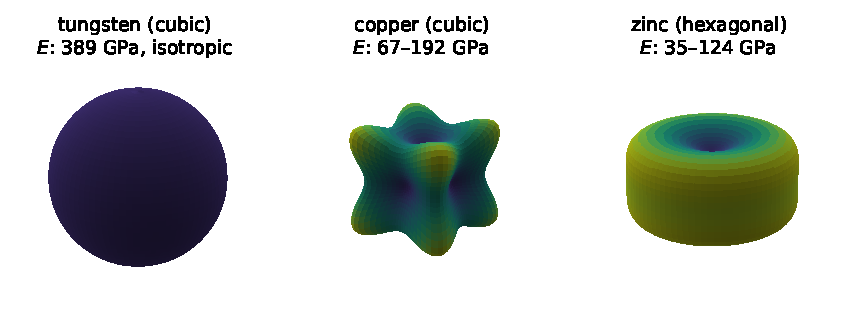
\includegraphics[width=0.92\textwidth]{figures/ch2/young_surface.pdf}
\caption{Directional Young's modulus: the surface $r=E(\vd)\,\vd$, coloured by
$E$ (each panel has its own scale). Tungsten is isotropic within the accuracy
of its compliances; copper is stiffest along the cube diagonals; zinc is
transversely isotropic about its hexagonal axis (vertical). Compliances
of~\cite{Nye1985}.}
\label{fig:el-young}
\end{figure}

\begin{gbox}{Isotropic elasticity}
\index{elasticity!isotropic}\index{Lam\'e constants@Lam\'e constants}\index{Young's modulus}\index{Poisson's ratio}\index{bulk modulus}%
\begin{gather}
  \bbC=\lambda\,\tI\otimes\tI+2\mu\,\bbI,\qquad
  \sig=\lambda(\tr\eps)\,\tI+2\mu\,\eps,\\
  \bbS=-\frac{\nu}{E}\,\tI\otimes\tI+\frac{1+\nu}{E}\,\bbI,\qquad
  \eps=-\frac{\nu}{E}(\tr\sig)\,\tI+\frac{1+\nu}{E}\,\sig,
\end{gather}
with $\bbI$ the symmetric fourth-order identity,
$I_{ijkl}=\tfrac12(\delta_{ik}\delta_{jl}+\delta_{il}\delta_{jk})$, so that
$C_{ijkl}=\lambda\delta_{ij}\delta_{kl}+\mu(\delta_{ik}\delta_{jl}+\delta_{il}\delta_{jk})$.
The Lam\'e constants $(\lambda,\mu)$ and the engineering constants
$(E,\nu)$ are related by
\begin{equation}\label{eq:lame}
  E=\frac{\mu(3\lambda+2\mu)}{\lambda+\mu},\quad
  \nu=\frac{\lambda}{2(\lambda+\mu)},\qquad
  \lambda=\frac{\nu E}{(1+\nu)(1-2\nu)},\quad
  \mu=\frac{E}{2(1+\nu)} ,
\end{equation}
and the bulk modulus is $K=\lambda+\tfrac23\mu=E/\bigl(3(1-2\nu)\bigr)$.
In matrix form~\eqref{eq:voigt}, $C_{1111}=\lambda+2\mu$, $C_{1122}=\lambda$,
$C_{2323}=\mu=\tfrac12(C_{1111}-C_{1122})$.
\end{gbox}

\subsection{Positive definiteness of \texorpdfstring{$\bbC$}{C}}
\index{material stability}\index{positive definiteness!of the elastic moduli}%
\begin{figure}[h]
\centering
\begin{tikzpicture}[>={Latex[length=2mm]},
  declare function={sg(\e)=2.6*(\e/2.8)*exp(1-\e/2.8);}]
  \draw[->] (0,0) -- (6.4,0) node[below left] {strain $\varepsilon$};
  \draw[->] (0,0) -- (0,3.3) node[above] {stress $\sigma$};
  \draw[cu,very thick,domain=0:2.8,samples=60] plot (\x,{sg(\x)});
  \draw[red!70!black,very thick,dashed,domain=2.8:6.1,samples=60] plot (\x,{sg(\x)});
  \draw[gray,densely dotted] (2.8,0) -- (2.8,2.6);
  \fill (2.8,2.6) circle (1.5pt);
  \node[cu,align=center,font=\small] at (1.0,3.05) {stable\\ $\dd\sigma\,\dd\varepsilon>0$};
  \node[red!70!black,align=center,font=\small] at (4.5,3.05) {unstable\\ $\dd\sigma\,\dd\varepsilon<0$};
  \draw[cu] (1.0,{sg(1.0)}) -- (1.5,{sg(1.0)}) node[midway,below,font=\scriptsize]{$\dd\varepsilon$}
     -- (1.5,{sg(1.5)}) node[midway,right,font=\scriptsize]{$\dd\sigma$};
  \draw[red!70!black] (4.5,{sg(4.5)}) -- (5.6,{sg(4.5)}) node[midway,above,font=\scriptsize]{$\dd\varepsilon$}
     -- (5.6,{sg(5.6)}) node[midway,right,font=\scriptsize]{$\dd\sigma$};
\end{tikzpicture}
\caption{Material stability. On the stable branch a strain increment needs
positive work, $\dd\sigma\,\dd\varepsilon>0$; beyond the peak the tangent
stiffness is negative and the response is unstable.}
\label{fig:stability}
\end{figure}
Positive definiteness of $\bbC$ and $\bbS$ is a condition of \emph{material
stability} (Figure~\ref{fig:stability}): the work needed to deform the
material is positive. For isotropic elasticity, split the strain into its
spherical and deviatoric parts, $\eps=\tfrac13(\tr\eps)\tI+\dev\eps$:
\begin{equation}\label{eq:iso-energy}
  \eps:\bbC:\eps=K\,(\tr\eps)^2+2\mu\,\dev\eps:\dev\eps .
\end{equation}
Hence $\bbC$ is positive definite iff $K>0$ and $\mu>0$: the three elementary
tests of Figure~\ref{fig:tests} have positive stiffness. Equivalently, $E>0$
and $-1<\nu<\tfrac12$ (Exercise~\ref{exo:posdef}).
\begin{figure}[h]
\centering
\begin{tikzpicture}[>={Latex[length=2mm]}]
 % tension: longer and thinner
 \begin{scope}
  \fill[gray!15] (-0.42,0) rectangle (0.42,2.6);
  \draw (-0.42,0) rectangle (0.42,2.6);
  \draw[cu,dashed] (-0.36,-0.15) rectangle (0.36,2.75);
  \draw[->,thick,cphi] (0,2.75) -- (0,3.35) node[above] {$F$};
  \draw[->,thick,cphi] (0,-0.15) -- (0,-0.75) node[below] {$F$};
  \node[font=\small,align=center] at (0,-1.6) {\sffamily tension\\ $E>0$};
 \end{scope}
 % torsion: a generator turns into a helix
 \begin{scope}[xshift=3.3cm]
  \fill[gray!15] (-0.45,0) rectangle (0.45,2.6);
  \draw (-0.45,0) -- (-0.45,2.6) (0.45,0) -- (0.45,2.6);
  \draw (0,2.6) ellipse (0.45 and 0.13);
  \draw (0.45,0) arc (0:-180:0.45 and 0.13);
  \draw[densely dashed] (0.45,0) arc (0:180:0.45 and 0.13);
  \draw[gray] (0,-0.13) -- (0,2.47);
  \draw[cu,thick,dashed] (0,-0.13) .. controls (0.12,1.0) and (0.3,1.8) .. (0.38,2.53);
  \draw[->,thick,cphi] (-0.6,3.0) arc (200:520:0.6 and 0.16);
  \draw[->,thick,cphi] (0.6,-0.45) arc (20:340:0.6 and 0.16);
  \node[cphi] at (0.95,3.15) {$M$};
  \node[font=\small,align=center] at (0,-1.6) {\sffamily torsion\\ $\mu>0$};
 \end{scope}
 % dilatation under hydrostatic pressure: the volume decreases
 \begin{scope}[xshift=6.8cm,yshift=1.3cm]
  \fill[gray!15] (0,0) circle (0.8);
  \draw (0,0) circle (0.8);
  \draw[cu,dashed] (0,0) circle (0.66);
  \foreach \a in {0,45,...,315}
    \draw[<-,thick,cphi] (\a:0.85) -- (\a:1.45);
  \node[cphi] at (1.45,1.1) {$p$};
  \node[font=\small,align=center] at (0,-2.9) {\sffamily dilatation\\ $K=\lambda+\tfrac23\mu>0$};
 \end{scope}
\end{tikzpicture}
\caption{The three elementary tests of isotropic elasticity (initial shape
in gray, deformed shape dashed): tension, torsion and uniform pressure. The
three stiffnesses $E$, $\mu$ and $K$ must be positive.}
\label{fig:tests}
\end{figure}

\paragraph{Negative Poisson's ratio.} The range $-1<\nu<\tfrac12$ is imposed
\index{auxetic material}\index{Poisson's ratio!negative}%
by stability, i.e.\ the positive definiteness of $\bbC$, not by
thermodynamics. Nothing forbids
$\nu<0$: \emph{auxetic} materials, mostly architected lattices and foams,
expand laterally when stretched.

%======================================================================
\section{Structure of the equations}\label{sec:el-structure}
\index{Tonti diagram!elasticity}\index{Navier equations}\index{admissible fields!kinematically}\index{admissible fields!statically}%
The equations of elasticity have the structure of the spring chain of
Chapter~\ref{ch:var} (Figure~\ref{fig:tonti-el}): the gradient operator
$\eps[\cdot]$ plays the role of $\mat{B}$, the divergence that of $\mat{B}\T$,
and $\bbC$ that of $\mat{C}$. Substituting, the displacement solves the
\emph{Navier equations}
\[
  \dive\bigl(\bbC:\eps[\vu]\bigr)+\vfD=\vzero,\qquad\text{isotropic:}\quad
  (\lambda+\mu)\nabla(\dive\vu)+\mu\Delta\vu+\vfD=\vzero .
\]
\begin{figure}[h]
\centering
\begin{tikzpicture}[node distance=1.2cm and 1.3cm]
  \node[smallbox,kin,minimum width=4.3cm] (u) {$\vu$, \quad $\vu=\vuD$ on $S_u$\\ \footnotesize displacement};
  \node[smallbox,stat,minimum width=4.3cm,right=3.6cm of u] (f) {$\dive\sig+\vfD=\vzero$ in $\Omega$,\ \ $\sig\vn=\vtD$ on $S_t$\\ \footnotesize body forces and tractions};
  \node[smallbox,kin,minimum width=4.3cm,below=of u] (e) {$\eps=\tfrac12(\nabla+\nabla\T)\vu$\\ \footnotesize strain};
  \node[smallbox,stat,minimum width=4.3cm,below=of f] (s) {$\sig=\bbC:\eps$\\ \footnotesize stress};
  \draw[arr] (u) -- (e) node[midway,left,font=\small]{$\eps[\cdot]$};
  \draw[arr] (e) -- (s) node[midway,below,font=\small]{$\bbC$};
  \draw[arr] (s) -- (f) node[midway,right,font=\small]{$-\dive$, \ $\cdot\,\vn$};
  \node[below=0.15cm of e,kinlab] {kinematically admissible: $\Kad(\vuD,S_u)$};
  \node[below=0.15cm of s,statlab] {statically admissible: $\Sad(\vfD,\vtD,S_t)$};
\end{tikzpicture}
\caption{Tonti diagram of linear elasticity. Left column (blue): kinematic
quantities, with the displacement prescribed on $S_u$; right column (green):
static quantities, with the balance equation and the prescribed tractions;
they are joined by the constitutive law. Compare with
Figures~\ref{fig:tonti-discrete} and~\ref{fig:tonti-diff}.}
\label{fig:tonti-el}
\end{figure}

The two columns define the two sets of admissible fields:
\begin{align*}
  \Kad(\vuD,S_u)&=\{\vv\ :\ \vv=\vuD\ \text{on }S_u\},\\
  \Sad(\vfD,\vtD,S_t)&=\{\tens{s}\ :\ \tens{s}=\tens{s}\T,\ \dive\tens{s}+\vfD=\vzero\ \text{in }\Omega,\
     \tens{s}\vn=\vtD\ \text{on }S_t\}.
\end{align*}
The solution is the field $\vu\in\Kad$ whose stress $\bbC:\eps[\vu]$ lies in
$\Sad$.

%======================================================================
\section{Virtual work: the weak form of the balance}\label{sec:el-vw}
\index{virtual power principle}\index{virtual work!continuum}\index{rigid body motion}%
For a virtual velocity (or displacement) field $\vv$ define the virtual
powers of the external, internal and inertial forces:
\[
  \mathcal P_e(\vv)=\int_\Omega\vf\cdot\vv\dd x+\int_{\partial\Omega}\vt\cdot\vv\dd s,\qquad
  \mathcal P_i(\vv)=-\int_\Omega\sig:\eps[\vv]\dd x,\qquad
  \mathcal P_a(\vv)=\int_\Omega\rho\,\ddot\vu\cdot\vv\dd x .
\]
\begin{gbox}{Principle of virtual power}
For every virtual velocity field $\vv$,
\begin{equation}\label{eq:pvp}
  \mathcal P_e(\vv)+\mathcal P_i(\vv)=\mathcal P_a(\vv).
\end{equation}
In statics $\mathcal P_a=0$. For every \emph{rigid} infinitesimal field
$\vv=\vect{a}+\vb\times\vx$, $\vect{a},\vb\in\R^3$, $\eps[\vv]=\vzero$ and
$\mathcal P_i(\vv)=0$.
\end{gbox}
The principle is equivalent to the local balance~\eqref{eq:balance} with the
boundary condition $\sig\vn=\vt$. Indeed, by Theorem~\ref{thm:ibp-tensor}
and the symmetry of $\sig$,
\[
  \int_\Omega\sig:\eps[\vv]\dd x=-\int_\Omega(\dive\sig)\cdot\vv\dd x
  +\int_{\partial\Omega}(\sig\vn)\cdot\vv\dd s ,
\]
and~\eqref{eq:pvp} for all $\vv$ is
$\displaystyle \int_\Omega(\dive\sig+\vf)\cdot\vv+\int_{\partial\Omega}(\vt-\sig\vn)\cdot\vv=0$.
This is the continuum version of $\vect{\sigma}\T\mat{B}\vu=\vf\T\vu$: the
divergence is the adjoint of the symmetric gradient.

\begin{gbox}{Adjoint and transpose}
\index{adjoint operator!of the gradient}\index{adjoint operator!boundary trace}%
The adjoint of the kinematic operator is a \emph{pair}: an operator in the
volume and a trace on the boundary,
\begin{align*}
  \int_\Omega\sig:\eps[\vv]\dd x&=\int_\Omega(-\dive\sig)\cdot\vv\dd x
  +\int_{S_t}(\sig\vn)\cdot\vv\dd s,\\
  \int_\Omega\vp\cdot\nabla v\dd x&=\int_\Omega(-\dive\vp)\,v\dd x
  +\int_{S_\varphi}(\vp\cdot\vn)\,v\dd s,
\end{align*}
for all $\vv$, $v$ vanishing on $S_u$. The adjoint of $\eps[\cdot]$ is $-\dive$
in $\Omega$ together with the traction $\sig\vn$ on $S_t$; the adjoint of
$\nabla$ is $-\dive$ in $\Omega$ together with the flux $\vp\cdot\vn$ on
$S_\varphi$. In the discrete setting both are contained in the single matrix
$\mat{B}\T$: interior rows give the balance of the internal nodes, rows of
boundary nodes give the nodal forces. On $S_u$ the test functions vanish,
and the trace there is the unknown reaction.
\end{gbox} Rigid motions do no
internal work; for a body without displacement constraints, choosing rigid
$\vv$ in~\eqref{eq:pvp} gives the global balance of forces and moments.

With the constitutive law, and $\vv$ restricted to fields vanishing on
$S_u$, the principle becomes the weak form of elasticity: find
$\vu\in\Kad(\vuD,S_u)$ such that
\begin{equation}\label{eq:el-weak}
  \int_\Omega\eps[\vu]:\bbC:\eps[\vv]\dd x=\int_\Omega\vfD\cdot\vv\dd x
  +\int_{S_t}\vtD\cdot\vv\dd s\qquad\forall\vv\in\Kad(\vzero,S_u).
\end{equation}

\paragraph{Existence: Korn's inequality.}
\index{Korn's inequality}\index{Lax--Milgram theorem!elasticity}%
For diffusion, coercivity came from the Poincar\'e inequality. In elasticity
the energy controls only the \emph{symmetric} part of $\nabla\vv$: the skew
part, an infinitesimal rotation, costs no energy. Positive definiteness of
$\bbC$ is therefore not enough by itself. The missing step is a classical
inequality of Korn.
\begin{gbox}{Korn's inequality and well-posedness of elasticity}
Let $\Omega$ be bounded, connected, with a Lipschitz boundary, and
$|S_u|>0$. There is a constant $c_K>0$ such that
\[
  \int_\Omega\eps[\vv]:\eps[\vv]\dd x\ \ge\ c_K\,\norm{\vv}^2_{H^1(\Omega)}
  \qquad\forall\vv\in\Kad(\vzero,S_u).
\]
With $\eps:\bbC:\eps\ge c_C\,\eps:\eps$ (for isotropy $c_C=\min(3K,2\mu)$, the smallest eigenvalue of $\bbC$,
Section~\ref{sec:el-moduli}), the form of~\eqref{eq:el-weak} is coercive with
constant $c_Cc_K$. It is continuous, and Lax--Milgram gives a unique solution
$\vu$ depending continuously on $(\vfD,\vtD,\vuD)$.
\end{gbox}
The constant $c_K$ depends on the shape of $\Omega$ and on $S_u$; it degrades
for slender bodies, which explains the stiff, badly conditioned systems of
thin structures. If $S_u=\emptyset$, the inequality holds only up to the rigid
motions: a solution exists if and only if the loads satisfy the global balance
of forces and moments, and it is unique up to a rigid motion. This is the
elastic counterpart of the Neumann problem of diffusion, unique up to a
constant (Exercise~\ref{exo:neumann}).

%======================================================================
\section{Energy principles}\label{sec:el-energy}
\index{energy!potential}\index{energy!complementary (elasticity)}\index{thermoelasticity}\index{initial stress}%
We include an initial stress $\sig_0$ and a thermal strain
$\talpha\,\theta^D$ (thermal expansion tensor $\talpha$, prescribed
temperature change $\theta^D$), so that
$\sig=\sig_0+\bbC:(\eps-\talpha\,\theta^D)$.

\begin{gbox}{Potential energy}
For $\vv\in\Kad(\vuD,S_u)$, the potential energy is the sum of an internal
and an external part, $\mathcal U_p=\mathcal U_i+\mathcal U_e$:
\begin{equation}\label{eq:Up}
  \mathcal U_p(\vv)=\int_\Omega\Bigl(\sig_0:\eps[\vv]+\tfrac12\eps[\vv]:\bbC:\eps[\vv]
  -\eps[\vv]:\bbC:\talpha\,\theta^D\Bigr)\dd x
  -\int_\Omega\vv\cdot\vfD\dd x-\int_{S_t}\vv\cdot\vtD\dd s .
\end{equation}
\end{gbox}

\begin{gbox}{Complementary energy}
For $\tens{s}\in\Sad(\vfD,\vtD,S_t)$, with
$\hat{\tens{s}}=\tens{s}-\sig_0+\bbC:\talpha\,\theta^D$,
\begin{equation}\label{eq:Uc}
  \mathcal U_p^\ast(\tens{s})=-\frac12\int_\Omega\hat{\tens{s}}:\bbS:\hat{\tens{s}}\dd x
  +\int_{S_u}\vuD\cdot(\tens{s}\vn)\dd s .
\end{equation}
\end{gbox}

\begin{gbox}{Extremal properties}
\index{minimum principle!potential energy}\index{maximum principle!complementary energy}\index{energy bounds}%
Let $(\vu,\eps,\sig)$ be the solution of a regular thermoelastic problem.
\begin{itemize}
\item $\vu$ \emph{minimizes} the potential energy over the kinematically
admissible fields: $\mathcal U_p(\vv)\ge\mathcal U_p(\vu)$ for all
$\vv\in\Kad(\vuD,S_u)$.
\item $\sig$ \emph{maximizes} the complementary energy over the statically
admissible fields: $\mathcal U_p^\ast(\sig)\ge\mathcal U_p^\ast(\tens{s})$ for
all $\tens{s}\in\Sad(\vfD,\vtD,S_t)$.
\item If $\sig_0=\vzero$ and $\theta^D=0$, the two values coincide:
$\mathcal U_p(\vu)=\mathcal U_p^\ast(\sig)$.
\end{itemize}
\end{gbox}
Hence, for any admissible pair,
$\mathcal U_p^\ast(\tens{s})\le\mathcal U_p^\ast(\sig)=\mathcal U_p(\vu)\le\mathcal U_p(\vv)$:
two-sided bounds on the energy, and on any quantity it controls
(Figure~\ref{fig:energy-scheme}). This is the duality of
Section~\ref{sec:var-dual} for elasticity.

\paragraph{Proof of the minimum principle.} For $\vv\in\Kad$, $\vv-\vu$
vanishes on $S_u$, and the weak form~\eqref{eq:el-weak} states that the
linear part of $\mathcal U_p(\vv)-\mathcal U_p(\vu)$ vanishes:
$D\mathcal U_p(\vu)(\vv-\vu)=0$. Therefore
\[
  \mathcal U_p(\vv)-\mathcal U_p(\vu)
  =\mathcal U_i(\vv)-\mathcal U_i(\vu)-D\mathcal U_i(\vu)(\vv-\vu)
  =\frac12\int_\Omega\eps[\vv-\vu]:\bbC:\eps[\vv-\vu]\dd x\ \ge0,
\]
by convexity of the internal energy, i.e.\ positive definiteness of $\bbC$
(Figure~\ref{fig:convexity}). Equality holds only if $\eps[\vv-\vu]=\vzero$,
i.e.\ $\vv-\vu$ is a rigid motion vanishing on $S_u$; if $S_u$ prevents rigid
motions, $\vv=\vu$. The maximum principle is proved in the same way with the
positive definiteness of $\bbS$; the equality of potentials follows from the
virtual work identity
$\displaystyle \int_\Omega\sig:\eps[\vu]=\int_\Omega\vfD\cdot\vu+\int_{S_t}\vtD\cdot\vu+\int_{S_u}(\sig\vn)\cdot\vuD$
(Exercise~\ref{exo:equality}).

\begin{figure}[h]
\centering
\begin{minipage}{0.45\textwidth}\centering
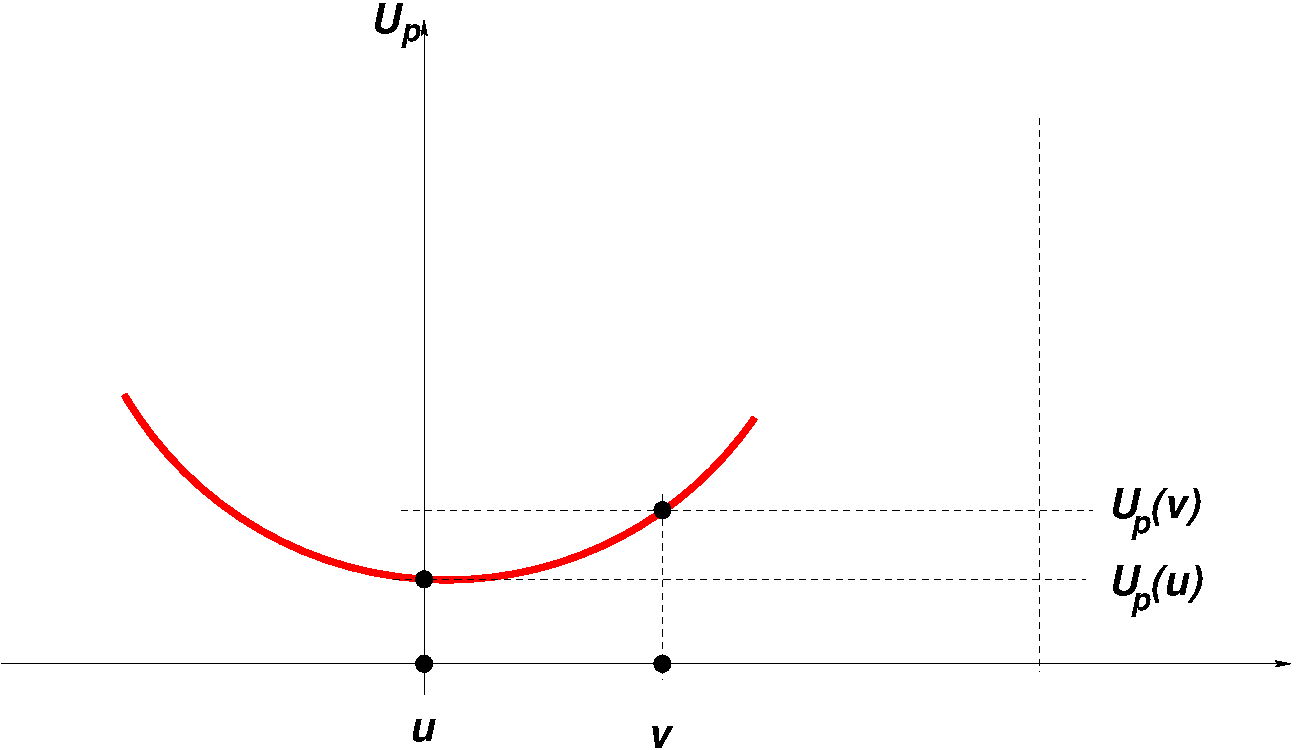
\includegraphics[width=0.9\textwidth]{figures/ch2/convex_minimum.pdf}
\end{minipage}\hfill
\begin{minipage}{0.45\textwidth}\centering
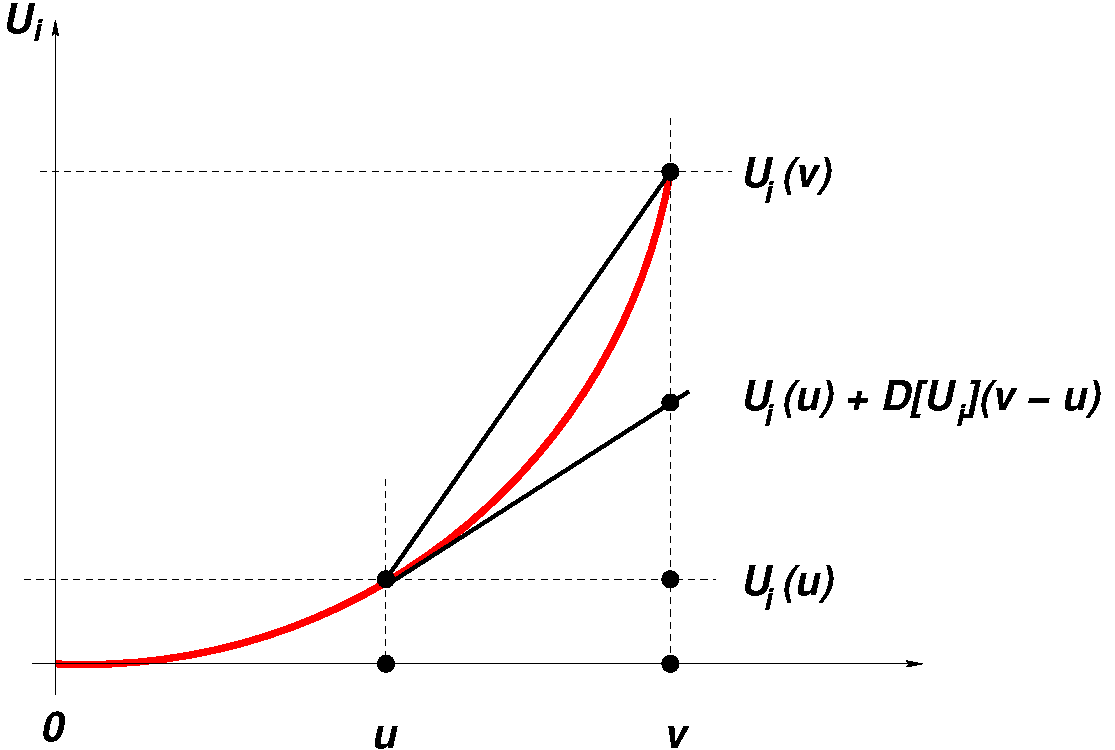
\includegraphics[width=0.9\textwidth]{figures/ch2/convex_du.pdf}
\end{minipage}
\caption{Left: the potential energy is minimal at $\vu$. Right: a convex
function lies above its tangent, $\mathcal U_i(\vv)\ge\mathcal U_i(\vu)+D\mathcal U_i(\vu)(\vv-\vu)$.}
\label{fig:convexity}
\end{figure}

\begin{figure}[h]
\centering
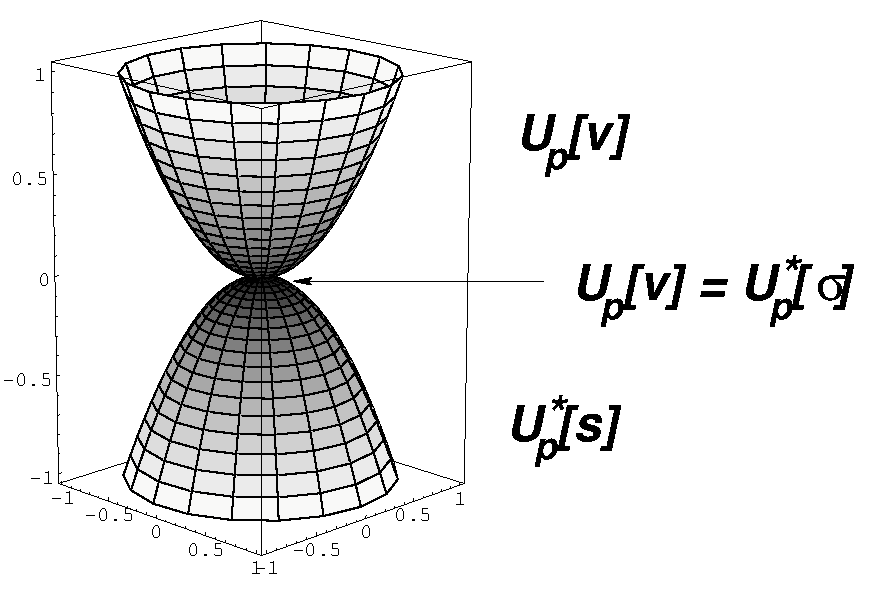
\includegraphics[height=6cm]{figures/ch2/energy_scheme.pdf}
\caption{The potential energy $\mathcal U_p[\vv]$ (a convex bowl over
kinematically admissible fields) and the complementary energy
$\mathcal U_p^\ast[\tens{s}]$ (a concave cap over statically admissible
fields) touch at the solution.}
\label{fig:energy-scheme}
\end{figure}

\subsection{The Lagrangian of the potential energy}\label{ssec:el-lagrangian}
\index{Lagrangian!potential energy}\index{Lagrange multiplier!reaction force}\index{thermoelasticity!Lagrangian}%
The minimum principle is posed on the constrained set $\Kad(\vuD,S_u)$.
Following~\cite{BonnetFrangi2007}, the constraint can be relaxed with a
Lagrange multiplier on $S_u$, which yields all the equations, including the
boundary conditions and the reactions, from a single stationarity condition.

\begin{gbox}{Lagrangian of thermoelasticity}
For unconstrained fields $\vv$ and multipliers $\vlambda$ on $S_u$,
\begin{multline}\label{eq:L-el}
  \mathcal L(\vv,\vlambda)=\int_\Omega\Bigl(\sig_0:\eps[\vv]
  +\tfrac12\bigl(\eps[\vv]-\talpha\theta^D\bigr):\bbC:\bigl(\eps[\vv]-\talpha\theta^D\bigr)\Bigr)\dd x\\
  -\int_\Omega\vfD\cdot\vv\dd x-\int_{S_t}\vtD\cdot\vv\dd s
  -\int_{S_u}\vlambda\cdot(\vv-\vuD)\dd s .
\end{multline}
The solution $(\vu,\vlambda)$ is a saddle point of $\mathcal L$: a minimum in
$\vv$ and a maximum in $\vlambda$.
\end{gbox}
\paragraph{Derivation of the equations.} Write
$\sig=\sig_0+\bbC:(\eps[\vu]-\talpha\theta^D)$. Stationarity with respect to
$\vlambda$ gives $\vu=\vuD$ on $S_u$. Stationarity with respect to $\vv$, in
every direction $\vw$, gives
\[
  \int_\Omega\sig:\eps[\vw]\dd x-\int_\Omega\vfD\cdot\vw\dd x
  -\int_{S_t}\vtD\cdot\vw\dd s-\int_{S_u}\vlambda\cdot\vw\dd s=0 .
\]
Integrating by parts with Theorem~\ref{thm:ibp-tensor},
\[
  \int_\Omega(-\dive\sig-\vfD)\cdot\vw\dd x+\int_{S_t}(\sig\vn-\vtD)\cdot\vw\dd s
  +\int_{S_u}(\sig\vn-\vlambda)\cdot\vw\dd s=0\qquad\forall\vw,
\]
hence the balance $\dive\sig+\vfD=\vzero$ in $\Omega$, the traction condition
$\sig\vn=\vtD$ on $S_t$, and $\vlambda=\sig\vn$ on $S_u$: the multiplier is
the traction exerted by the support, the reaction, with its sign. This is
the reason for the minus sign in front of the constraint
in~\eqref{eq:L-el}; the discrete system~\eqref{eq:saddle} keeps the same
convention. The constitutive law,
with its thermal and initial-stress terms, is contained in the definition of
the energy density.

The Lagrangian of diffusion, built in the same way, is given in
Section~\ref{ssec:diff-lagrangian}.

\paragraph{Remark: two-field Lagrangians.} Relaxing also the constitutive law,
with the stress as an independent field, gives the Hellinger--Reissner
functional, and relaxing the compatibility $\eps=\eps[\vu]$ the Hu--Washizu
functional~\cite{BonnetFrangi2007}. They are the basis of mixed finite
elements, used for incompressible materials.

%======================================================================
\section{Approximate solutions: from Ritz--Galerkin to finite elements}\label{sec:el-ritz}
\index{Ritz--Galerkin method}\index{approximate solution}%
Closed-form solutions exist only for simple geometries. The equations can be
solved approximately by finite differences, by series expansions, or by the
energy principle: the Ritz--Rayleigh/Galerkin technique, of which finite
elements are a particular case.

\subsection{The Ritz--Galerkin method}
\begin{gbox}{Ritz--Galerkin approximation}
The approximate solution $\vu^A$ minimizes the potential energy over a
finite-dimensional subset $\Kad_A\subset\Kad(\vuD,S_u)$ of admissible
displacement fields:
\[
  \vu^A=\argmin_{\vv\in\Kad_A}\mathcal U_p[\vv].
\]
\end{gbox}
\begin{figure}[h]
\centering
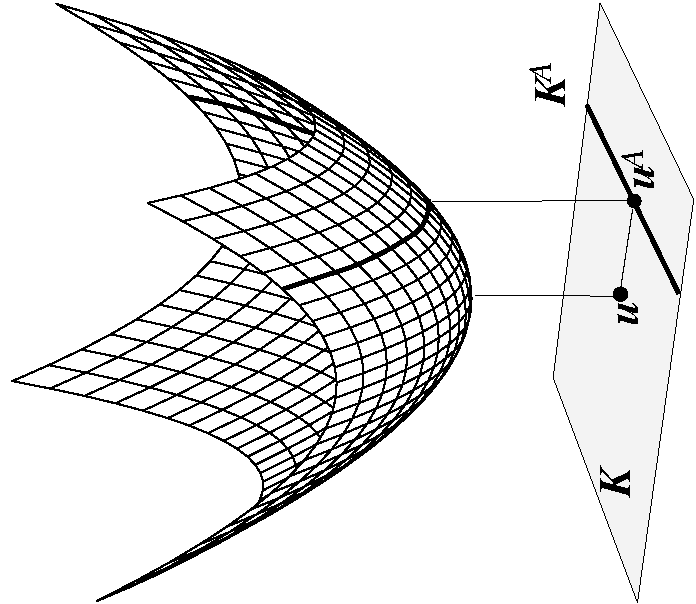
\includegraphics[angle=-90,width=0.38\textwidth]{figures/ch2/approximate_solution.pdf}
\caption{The Ritz approximation minimizes the same energy on a smaller set
$\Kad^A\subset\Kad$; by the minimum principle,
$\mathcal U_p(\vu)\le\mathcal U_p(\vu^A)$.}
\label{fig:ritz}
\end{figure}
Write the trial fields as combinations of $M$ given fields with unknown
coefficients:
\[
  \vv[\vect{\alpha}]=\sum_{m=1}^M\alpha_m\vw_m,\qquad
  \vect{\alpha}=(\alpha_1,\dots,\alpha_M)\in\R^M .
\]
For homogeneous data on $S_u$ (otherwise add a fixed field satisfying
$\vv=\vuD$), the energy is a quadratic function of $\vect{\alpha}$,
\[
  \mathcal U_p(\vv[\vect{\alpha}])=\tfrac12\vect{\alpha}\T\mat{K}\vect{\alpha}-\vect{\beta}\T\vect{\alpha},
\]
\[
  K_{m\ell}=\int_\Omega\eps[\vw_m]:\bbC:\eps[\vw_\ell]\dd x,\qquad
  \beta_m=\int_\Omega\vfD\cdot\vw_m+\int_{S_t}\vtD\cdot\vw_m .
\]
The stiffness matrix $\mat{K}$ is symmetric (major symmetry of $\bbC$) and
positive definite (positivity of $\bbC$, independent $\vw_m$ and no rigid
motion). By Theorem~\ref{thm:min-discrete} the minimum is the solution of
\[
  \mat{K}\vect{\alpha}=\vect{\beta},\qquad
  \vu^A=\sum_{m=1}^M\alpha_m\vw_m .
\]

\subsection{Imposed displacements as constraints}\label{ssec:ritz-lagrange}
\index{Lagrange multiplier!imposed displacements}\index{reaction forces}%
Instead of building the boundary conditions into the trial fields, write
them as linear constraints on the unknowns, $\mat{P}\vu=\vuD$, and minimize
the potential energy subject to them (Section~\ref{sec:var-lagrange}). As in
the continuous Lagrangian~\eqref{eq:L-el}, the constraint enters with a minus
sign. The solution is the saddle point of
\[
  \mathcal L(\vu,\vlambda)=\tfrac12\vu\T\mat{K}\vu-\mat{F}\T\vu-\vlambda\T(\mat{P}\vu-\vuD),
  \qquad
  \frac{\partial\mathcal L}{\partial\vu}=\vzero,\quad
  \frac{\partial\mathcal L}{\partial\vlambda}=\vzero,
\]
that is
\begin{equation}\label{eq:saddle}
  \begin{bmatrix}\mat{K}&-\mat{P}\T\\ -\mat{P}&\mat{0}\end{bmatrix}
  \begin{bmatrix}\vu\\ \vlambda\end{bmatrix}=
  \begin{bmatrix}\mat{F}\\ -\vuD\end{bmatrix}.
\end{equation}
The first line reads $\mat{K}\vu=\mat{F}+\vect{r}$ with $\vect{r}=\mat{P}\T\vlambda$:
the multipliers are the reaction forces at the constrained degrees of freedom,
with their sign (Exercise~\ref{exo:lagrange-el}). The matrix is symmetric but
indefinite. $\mat{K}$ alone may be singular, since the supports are now in
$\mat{P}$. If $\mat{K}$ is positive definite on the kernel of $\mat{P}$ and
the constraints are independent, the solution is unique. Cast3M, for instance, imposes
displacement conditions this way.

\subsection{Which trial functions?}
\index{conditioning}\index{trial functions}%
\begin{itemize}
\item \emph{Global bases} of $L^2(\Omega)$. Polynomials give a full,
badly conditioned matrix $\mat{K}$: its eigenvalues spread over many orders of
magnitude as the degree grows, and the numerical inversion becomes unstable
(Exercise~\ref{exo:conditioning}). Trigonometric functions are suited only to
particular domains, and $\mat{K}$ is still full.
\item \emph{Finite elements}: piecewise polynomials on a partition of the
domain, continuous across the subdomains. The matrix is sparse and well
conditioned.
\item \emph{Isogeometric analysis}~\cite{HughesCottrellBazilevs2005,CottrellHughesBazilevs2009}:
\index{isogeometric analysis}\index{NURBS}%
the trial functions are the B-splines or NURBS that describe the exact CAD
geometry, smoother than standard elements ($C^{p-1}$ for degree $p$). They
are presented and compared with finite elements in
Section~\ref{sec:var-iga}.
\end{itemize}

\subsection{Finite elements}
\index{finite element method}\index{mesh}%
The finite element method is the Ritz--Galerkin method with a particular
choice of $\vw_m$: the domain $\Omega$ is approximated by a mesh $\Omega_h$
of elements, $\Omega_h\to\Omega$ as $h\to0$, and the unknowns are the nodal
values of the displacement,
\[
  \vu_h(\vx)=\sum_{m}u_i(\vx_m)\,w_m(\vx)\,\ve_i ,
\]
where $w_m$ is the shape function of node $m$: equal to $1$ at node $m$, $0$ at
the other nodes, polynomial on each element (Figure~\ref{fig:fem}).
\begin{figure}[h]
\centering
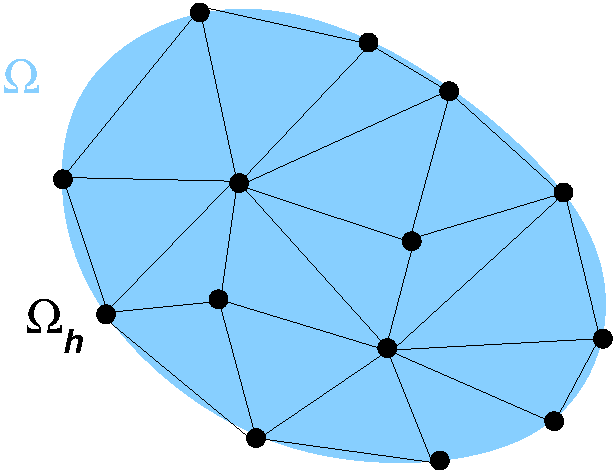
\includegraphics[width=0.3\textwidth]{figures/ch2/fem_mesh.pdf}\qquad\qquad
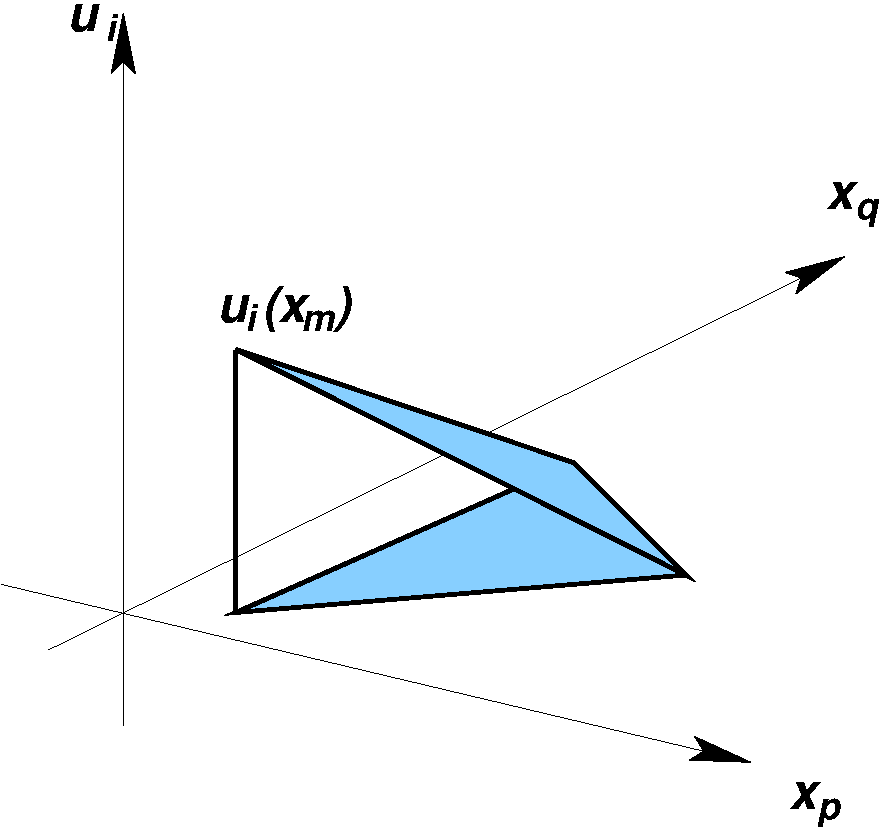
\includegraphics[width=0.36\textwidth]{figures/ch2/fem_element.pdf}
\caption{Left: a mesh $\Omega_h$ of the domain $\Omega$. Right: the shape
function of a node, linear on each triangle.}
\label{fig:fem}
\end{figure}

\paragraph{Shape functions.}
\index{finite element method!shape functions}\index{Hermite cubics}%
\begin{itemize}
\item \emph{Linear elements in one dimension:} $w=a+bx$; the unknowns are the
nodal values.
\item \emph{Cubic elements in one dimension} (Hermite cubics):
$w=a+bx+cx^2+dx^3$; the unknowns are the nodal values and slopes (beams).
Splines are not defined by nodal values alone and do not qualify as finite
elements in the sense of Ciarlet (Section~\ref{sec:var-bsplines}).
\item \emph{Bilinear elements on rectangles:} $w=a+bx+cy+dxy$.
\item \emph{Triangles:} linear, $w=a+bx+cy$, with nodes at the vertices;
quadratic, $w=a+bx+cy+dx^2+exy+fy^2$, with nodes at the vertices and the
mid-edges (Figure~\ref{fig:shape}).
\end{itemize}
\begin{figure}[h]
\centering
\begin{tabular}{ccc}
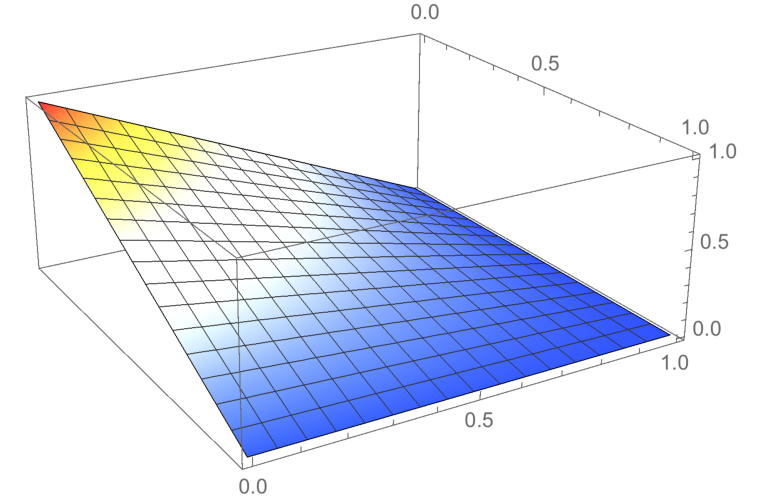
\includegraphics[height=2.4cm]{figures/ch2/P1_rectangle.pdf} &
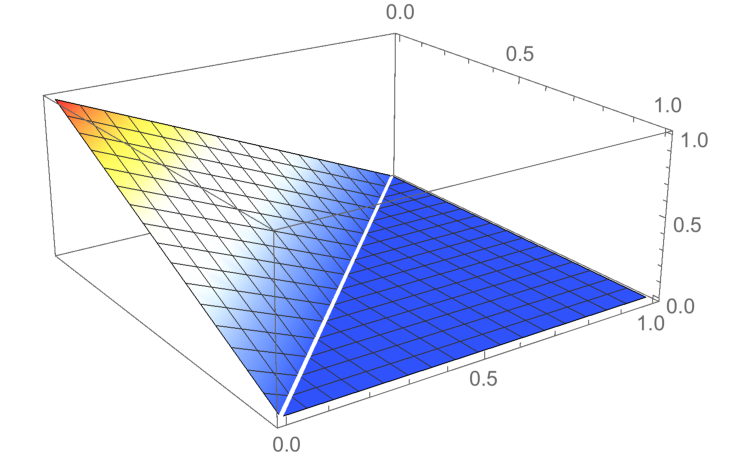
\includegraphics[height=2.4cm]{figures/ch2/P1_triangle.pdf} &
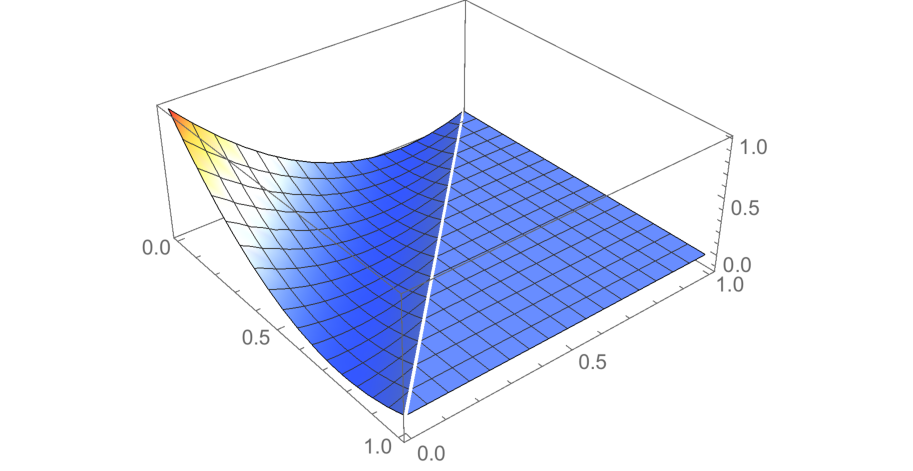
\includegraphics[height=2.4cm]{figures/ch2/P2_triangle.pdf}\\
{\small bilinear, rectangle} & {\small linear, $w=1-x-y$} & {\small quadratic, $w=(1-x-y)(1-2x-2y)$}
\end{tabular}
\caption{Shape functions of the node at the origin for three elements.}
\label{fig:shape}
\end{figure}

\paragraph{Numerical integration with Gauss points.}
\index{finite element method!Gauss points}\index{Gauss quadrature}%
The stiffness matrix is the sum of element contributions,
$\mat{K}=\sum_e\mat{K}_e$, each assembled at the rows and columns of the nodes
of element $e$. Each element is the image of a reference element
$\hat\Omega$ (the segment $[-1,1]$, the square $[-1,1]^2$, the unit triangle) by
a map $\vx(\vxi)$ with Jacobian matrix $\mat{J}=\partial\vx/\partial\vxi$
(Figure~\ref{fig:refmap}). In the \emph{isoparametric} map the geometry is
\index{isoparametric element}\index{Jacobian of the element map}%
interpolated like the displacement, $\vx(\vxi)=\sum_aN_a(\vxi)\,\vx_a$, with
the shape functions $N_a$ of the reference element and the nodes $\vx_a$. The
columns of $\mat{J}$ are the tangent vectors to the coordinate lines, and the
volume element is $\dd x=\det\mat{J}\dd\xi$. The map must be one-to-one,
$\det\mat{J}>0$ in the element: a badly distorted quadrilateral is rejected by
the code. The integral is computed on the reference element by a quadrature
rule:
\[
  \mat{K}_e=\int_{\Omega_e}\mat{B}\T\mat{C}\mat{B}\dd x
  =\int_{\hat\Omega}\mat{B}\T\mat{C}\mat{B}\,\det\mat{J}\dd\xi
  \approx\sum_{g=1}^{n_g}w_g\,\mat{B}\T(\vxi_g)\,\mat{C}\,\mat{B}(\vxi_g)\,\det\mat{J}(\vxi_g).
\]
The points $\vxi_g$ and weights $w_g$ of Gauss--Legendre quadrature are chosen
so that $n$ points integrate exactly the polynomials of degree $2n-1$ on
$[-1,1]$: one point $\xi=0$, $w=2$ (degree 1); two points
$\xi=\pm1/\sqrt3$, $w=1$ (degree 3); three points $0,\pm\sqrt{3/5}$ with
weights $\tfrac89,\tfrac59$ (degree 5). On quadrilaterals the rule is the
tensor product, $2\times2$ points for bilinear elements. On triangles, one
point at the centroid integrates linear functions, and the three points of
Figure~\ref{fig:gauss}, $(\tfrac16,\tfrac16)$, $(\tfrac23,\tfrac16)$,
$(\tfrac16,\tfrac23)$ with weights $\tfrac16$, integrate quadratics. The rule is
chosen to integrate the stiffness exactly for affine elements; fewer points
(reduced integration) soften the element, and too few produce spurious
zero-energy modes. The Gauss points are where the strains and stresses are
computed; for nonlinear materials they are also where the internal variables
(plastic strain, damage) are stored and the constitutive law is integrated,
which is the subject of the next part of the course.
\begin{figure}[h]
\centering
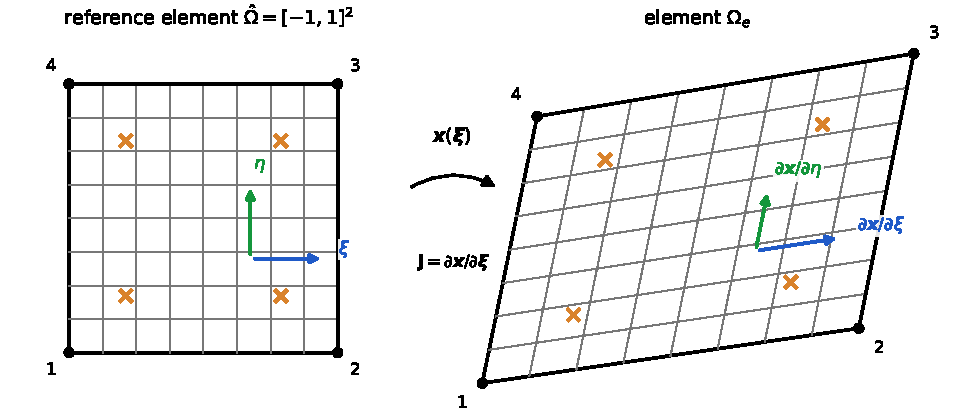
\includegraphics[width=0.85\textwidth]{figures/ch2/reference_map.pdf}
\caption{The isoparametric map $\vx(\vxi)=\sum_aN_a(\vxi)\,\vx_a$ of a
bilinear quadrilateral. The coordinate lines of the reference square are
mapped to straight lines of the element, no longer parallel; the columns of
$\mat{J}=\partial\vx/\partial\vxi$ are their tangent vectors. Crosses: the
$2\times2$ Gauss points and their images.}
\label{fig:refmap}
\end{figure}

\paragraph{Matrix structure.} The discrete equations reproduce the Tonti
\index{Tonti diagram!finite elements}\index{finite element method!Gauss points}%
diagram (Figure~\ref{fig:tonti-fem}):
\[
  \bigl(\mat{B}\T\mat{C}\mat{B}\bigr)\,\mat{u}=\mat{F},\qquad \mat{P}\mat{u}=\mat{u}^D,
\]
where $\mat{u}$ collects the nodal displacements, $\mat{B}$ computes the
strains from them, $\mat{C}$ is the matrix of $\bbC$ and $\mat{F}$ collects the
nodal forces equivalent to $\vfD$ and $\vtD$. Strains and stresses are
computed at the Gauss points of each element, where the integrals are
evaluated numerically (Figure~\ref{fig:gauss}).
\begin{figure}[h]
\centering
\begin{tikzpicture}[node distance=1.0cm and 1.1cm]
  \node[tinybox,kin,text width=3.2cm,minimum width=3.5cm] (u) {$\mat{u}$, \ $\mat{P}\mat{u}=\mat{u}^D$\\ \scriptsize nodal displacements};
  \node[tinybox,stat,text width=3.2cm,minimum width=3.5cm,right=4.2cm of u] (f) {$\mat{F}$\\ \scriptsize nodal forces};
  \node[tinybox,kin,text width=3.2cm,minimum width=3.5cm,below=of u] (e) {$\mat{e}=\mat{B}\mat{u}$\\ \scriptsize strains at Gauss points};
  \node[tinybox,stat,text width=3.2cm,minimum width=3.5cm,below=of f] (s) {$\mat{s}=\mat{C}\mat{e}$\\ \scriptsize stresses at Gauss points};
  \draw[arr] (u) -- (e) node[midway,left,font=\small]{$\mat{B}$};
  \draw[arr] (e) -- (s) node[midway,below,font=\small]{$\mat{C}$};
  \draw[arr] (s) -- (f) node[midway,right,font=\small]{$\mat{B}\T$};
  \node[below=0.15cm of e,kinlab] {kinematic};
  \node[below=0.15cm of s,statlab] {static};
\end{tikzpicture}
\caption{The discrete Tonti diagram of the finite element method; compare
with Figures~\ref{fig:tonti-discrete} and~\ref{fig:tonti-el}.}
\label{fig:tonti-fem}
\end{figure}
\begin{figure}[h]
\centering
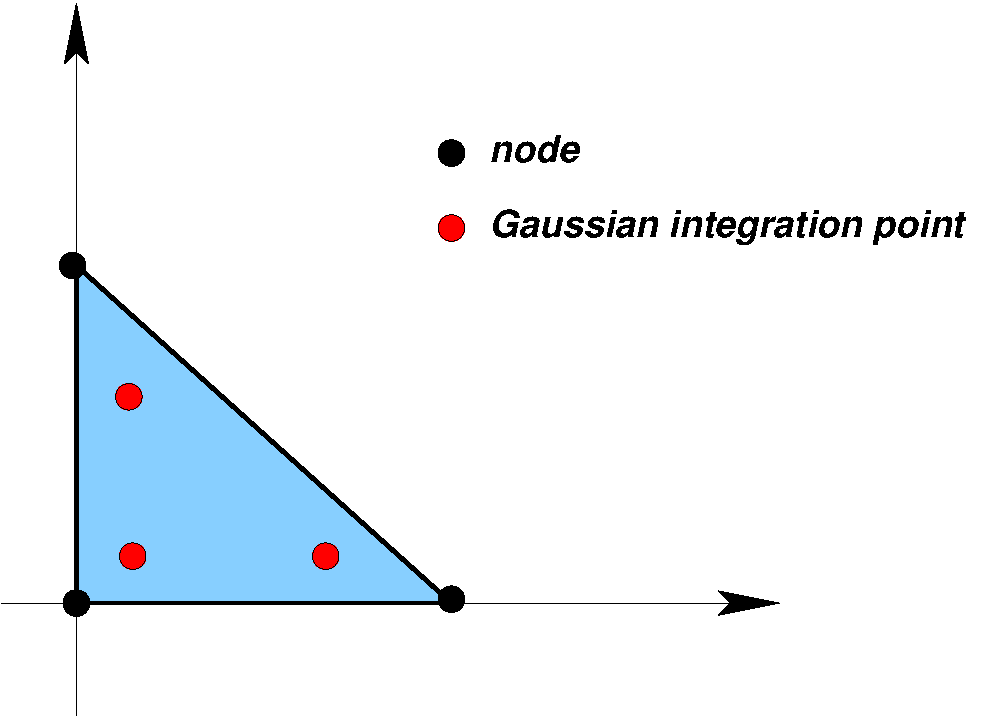
\includegraphics[width=0.45\textwidth]{figures/ch2/fem_point_gauss.pdf}
\caption{Nodes, where the displacements live, and Gauss points, where strains
and stresses are computed: $[\vu]\to\mat{B}\to[\eps]$ and
$[\sig]\to\mat{B}\T\to[\vf]$.}
\label{fig:gauss}
\end{figure}

\paragraph{A test case: the plate with a hole.} A finite element code is
\index{Kirsch problem}\index{stress concentration}%
checked against closed-form solutions. The classical one is the infinite
plate with a circular hole under a remote tension $\sigma$, solved by
Kirsch~\cite{Kirsch1898}: the hoop stress on the hole reaches $3\sigma$, a
stress concentration factor of $3$ whatever the radius. A small program with
linear triangles recovers it within $1\%$ with a few thousand unknowns,
provided the mesh is refined near the hole (Exercise~\ref{exo:kirsch},
Figure~\ref{fig:kirsch}).

%======================================================================
\framepart{Summary}
\begin{gbox*}
\begin{itemize}
  \item \textbf{The same structure} appears in all frameworks: discrete
  springs, diffusion, elasticity, finite elements (Table~\ref{tab:diff-el},
  Figures~\ref{fig:tonti-diff}, \ref{fig:tonti-el} and~\ref{fig:tonti-fem}):
  kinematic quantities and data (blue), static quantities and data (green),
  joined by the material law $\tk$ or $\bbC$.
  \item \textbf{Adjoint and transpose.} The adjoint of $\nabla$ and of
  $\eps[\cdot]$ is the pair formed by $-\dive$ in $\Omega$ and the boundary
  trace $\cdot\,\vn$ on $S_\varphi$ or $S_t$, the flux or the traction on the
  boundary. It corresponds to the transpose matrix $\mat{B}\T$; virtual work
  expresses this duality.
  \item \textbf{The Lagrangian} of the potential energy, with a multiplier
  for the imposed displacements or potentials, yields all the equations at
  once; the multiplier is the reaction (traction or flux) on $S_u$.
  \item \textbf{Elastic moduli.} $\bbC$ has minor and major symmetries
  ($21$ moduli in general, $2$ for isotropy) and must be positive definite:
  $K>0$, $\mu>0$, i.e.\ $E>0$ and $-1<\nu<\tfrac12$.
  \item \textbf{Uniqueness} follows from convexity, i.e.\ the positive
  definiteness of the energy, and from the displacement boundary conditions,
  which eliminate rigid motions.
  \item \textbf{Two energy principles} bound the solution from both sides;
  the Ritz--Galerkin and finite element methods minimize the potential energy
  on a finite-dimensional space, and imposed displacements can be enforced by
  Lagrange multipliers, the reactions.
\end{itemize}
\end{gbox*}

%======================================================================
\framepart{Exercises}\label{sec:el-exo}

\framesub{Short questions}
No documents, no computer: each question needs a few lines of computation.

\exercise{Boundary conditions}\label{exo:q-bc}
\index{boundary condition!elasticity}%
A cube $[0,a]^3$ rests on a frictionless rigid table, the plane $x_3=0$. A
uniform pressure $p$ acts on its top face; the lateral faces are free. Write
the boundary conditions on each face. Is the solution unique?
\begin{solution}
Bottom face: $u_3=0$ and $\sigma_{13}=\sigma_{23}=0$ (frictionless contact). Top
face: $\sig\vn=-p\,\ve_3$, i.e.\ $\sigma_{33}=-p$, $\sigma_{13}=\sigma_{23}=0$.
Lateral faces: $\sig\vn=\vzero$. The stress is unique,
$\sig=-p\,\ve_3\otimes\ve_3$. The displacement is unique up to the rigid
motions allowed by $u_3=0$: the translations along $\ve_1$, $\ve_2$ and the
rotation about $\ve_3$. Fixing three components at two points of the bottom
face removes them.
\end{solution}

\exercise{Engineering constants}\label{exo:q-constants}
A steel has $E=200$\,GPa and $\nu=0.25$. (a) Compute $\lambda$, $\mu$ and $K$.
(b) A bar carries a uniaxial stress $\sigma=100$\,MPa. Compute
$\varepsilon_{11}$, $\varepsilon_{22}$ and the relative change of volume.
\begin{solution}
(a) $\lambda=\nu E/\bigl((1+\nu)(1-2\nu)\bigr)=80$\,GPa,
$\mu=E/\bigl(2(1+\nu)\bigr)=80$\,GPa, $K=E/\bigl(3(1-2\nu)\bigr)=133$\,GPa.
(b) $\varepsilon_{11}=\sigma/E=5\times10^{-4}$,
$\varepsilon_{22}=\varepsilon_{33}=-\nu\sigma/E=-1.25\times10^{-4}$, and
$\tr\eps=(1-2\nu)\sigma/E=\sigma/(3K)=2.5\times10^{-4}$.
\end{solution}

\exercise{Is this material stable?}\label{exo:q-stable}
\index{auxetic material}%
A polymer foam is measured with $E=1$\,MPa and $K=0.2$\,MPa. Compute $\nu$
and $\mu$. Is the elastic energy positive definite?
\begin{solution}
$K=E/\bigl(3(1-2\nu)\bigr)$ gives $1-2\nu=E/(3K)=\tfrac53$, so $\nu=-\tfrac13$.
Then $\mu=E/\bigl(2(1+\nu)\bigr)=0.75$\,MPa. Since $K>0$ and $\mu>0$, the energy
is positive definite~\eqref{eq:iso-energy}: the foam is stable, and auxetic.
\end{solution}

\exercise{Why Korn?}\label{exo:q-korn}
\index{Korn's inequality}%
Take $\vv=\omega\,\ve_3\times\vx$ on the unit cube. Compute $\eps[\vv]$ and
$\nabla\vv$. Why is the positive definiteness of $\bbC$ not enough to make the
elastic form coercive on $H^1(\Omega)^3$? What changes when $|S_u|>0$?
\begin{solution}
$\vv=\omega(-x_2,x_1,0)$, so $\nabla\vv=\omega(\ve_2\otimes\ve_1-\ve_1\otimes\ve_2)$
is skew and $\eps[\vv]=\vzero$. The energy vanishes while
$\norm{\vv}_{H^1}>0$: no inequality $a(\vv,\vv)\ge c\norm{\vv}^2_{H^1}$ can hold
on $H^1(\Omega)^3$. If $\vv=\vzero$ on a part $S_u$ of positive area, the only
rigid motion allowed is zero, and Korn's inequality restores coercivity.
\end{solution}

\exercise{Is this crystal isotropic?}\label{exo:q-zener}
\index{Zener ratio}%
With Table~\ref{tab:el-stiffness}, compute the Zener ratio
$A=2c_{44}/(c_{11}-c_{12})$ of aluminium and of tungsten. For tungsten,
deduce $E$ and $\nu$ from $s_{11}=0.257$ and $s_{12}=-0.073$, in
$10^{-11}\,\mathrm{Pa}^{-1}$.
\begin{solution}
Aluminium: $A=56/46=1.22$, mildly anisotropic. Tungsten: $A=304/303=1.00$,
isotropic. Then $E=1/s_{11}=389$\,GPa and $\nu=-s_{12}/s_{11}=0.28$. Check:
$\mu=E/\bigl(2(1+\nu)\bigr)=152$\,GPa$\,=c_{44}$.
\end{solution}

\exercise{Weak form of a bar}\label{exo:q-weak}
\index{weak form!diffusion}%
Write the weak form of $-(ku')'=f$ on $(0,L)$, with $u(0)=u_0$ and
$k\,u'(L)=\varphi$. Which condition is essential, which is natural? Which
energy does $u$ minimize?
\begin{solution}
Multiply by $v$ with $v(0)=0$ and integrate by parts:
$\displaystyle \int_0^Lku'v'\dd x=\int_0^Lfv\dd x+\varphi\,v(L)$ for all such $v$, with
$u(0)=u_0$. The condition $u(0)=u_0$ is essential (it defines the space); the
flux $\varphi$ is natural (it enters the right-hand side). The solution
minimizes
$\displaystyle J(v)=\int_0^L\tfrac12k(v')^2\dd x-\int_0^Lfv\dd x-\varphi\,v(L)$ over
$v(0)=u_0$.
\end{solution}

\exercise{One spring, one multiplier}\label{exo:q-saddle}
\index{Lagrange multiplier!reaction force}%
A spring of stiffness $k$ joins a fixed point to a node loaded by a force $F$.
The displacement of the node is imposed, $u=\uD$, by a Lagrange multiplier as
in~\eqref{eq:saddle}. Write the $2\times2$ system, solve it and interpret
$\lambda$.
\begin{solution}
\[
\begin{bmatrix}k&-1\\-1&0\end{bmatrix}\begin{bmatrix}u\\ \lambda\end{bmatrix}
=\begin{bmatrix}F\\ -\uD\end{bmatrix}.
\]
The second line gives $u=\uD$, the first
$\lambda=k\uD-F$. The multiplier is the reaction $r=\lambda$: the support adds
the force $k\uD-F$ to $F$ to balance the spring force $k\uD$. If $F=k\uD$ no
reaction is needed.
\end{solution}

\exercise{A hole under biaxial loads}\label{exo:q-hole}
\index{stress concentration}%
Under a remote tension $\sigma$ along $\ve_1$, the hoop stress on a circular
hole in an infinite plate is $\sigma_{\theta\theta}=\sigma(1-2\cos2\theta)$
(Exercise~\ref{exo:kirsch}). By superposition, find $\sigma_{\theta\theta}$ on
the hole under (a) an equibiaxial tension $\sigma$ along $\ve_1$ and $\ve_2$;
(b) a pure shear, $\sigma$ along $\ve_1$ and $-\sigma$ along $\ve_2$. Give the
stress concentration factor in each case.
\begin{solution}
A tension along $\ve_2$ is the tension along $\ve_1$ rotated by $\tfrac\pi2$:
$\theta\to\theta-\tfrac\pi2$ changes $\cos2\theta$ into $-\cos2\theta$, so
it gives $\sigma(1+2\cos2\theta)$. (a) The sum is $2\sigma$, uniform on the
hole: factor $2$. (b) The difference is $-4\sigma\cos2\theta$: factor $4$. A
hole is most harmful in shear.
\end{solution}

\exercise{Zero-energy modes}\label{exo:q-modes}
\index{hourglass mode}%
A four-node quadrilateral in plane elasticity has $8$ degrees of freedom.
With one Gauss point, what is the largest possible rank of its stiffness
matrix? How many zero-energy modes does it have, and how many are spurious?
Same questions with $2\times2$ Gauss points.
\begin{solution}
With one point, $\mat{K}_e=w\,\mat{B}\T\mat{C}\mat{B}\det\mat{J}$ with $\mat{B}$ of
size $3\times8$: the rank is at most $3$. At least $8-3=5$ modes have zero
energy: $3$ rigid motions and $2$ spurious hourglass modes
(Exercise~\ref{exo:gauss}). With $2\times2$ points the rank is $8-3=5$: only
the rigid motions remain.
\end{solution}

\framesub{Elastic moduli and energy principles}

\exercise{Lam\'e and engineering constants}\label{exo:lame}
(a) From $\sig=\lambda(\tr\eps)\tI+2\mu\eps$, compute the response to a
uniaxial stress $\sig=\sigma\,\ve_1\otimes\ve_1$ and derive $E$ and $\nu$ in
terms of $\lambda,\mu$. (b) Derive the bulk modulus $K$ from a hydrostatic
stress $\sig=-p\tI$. (c) Invert the law and check the expression of $\bbS$.
\begin{solution}
(a) Taking the trace, $\tr\sig=(3\lambda+2\mu)\tr\eps$, so
$\displaystyle \eps=\frac{1}{2\mu}\bigl(\sig-\frac{\lambda}{3\lambda+2\mu}(\tr\sig)\tI\bigr)$.
For uniaxial stress, $\displaystyle \varepsilon_{11}=\frac{\lambda+\mu}{\mu(3\lambda+2\mu)}\sigma$
and $\displaystyle \varepsilon_{22}=-\frac{\lambda}{2\mu(3\lambda+2\mu)}\sigma$, so
$E=\sigma/\varepsilon_{11}=\mu(3\lambda+2\mu)/(\lambda+\mu)$ and
$\nu=-\varepsilon_{22}/\varepsilon_{11}=\lambda/(2(\lambda+\mu))$.
(b) $\tr\eps=-3p/(3\lambda+2\mu)$, so $K=-p/\tr\eps=\lambda+\tfrac23\mu$.
(c) Substituting $\displaystyle \frac1{2\mu}=\frac{1+\nu}{E}$ and
$\displaystyle \frac{\lambda}{2\mu(3\lambda+2\mu)}=\frac{\nu}{E}$ in (a) gives
$\displaystyle \eps=\frac{1+\nu}{E}\sig-\frac{\nu}{E}(\tr\sig)\tI$, i.e.\ the expression of
$\bbS$ in the box.
\end{solution}

\exercise{Positive definiteness of isotropic elasticity}\label{exo:posdef}
\index{incompressibility}%
(a) Prove~\eqref{eq:iso-energy}. (b) Show that $\bbC$ is positive definite iff
$K>0$ and $\mu>0$. (c) Show that this is equivalent to $E>0$ and
$-1<\nu<\tfrac12$. What happens as $\nu\to\tfrac12$?
\begin{solution}
(a) With $\eps=\tfrac13(\tr\eps)\tI+\dev\eps$ and $\tr\dev\eps=0$:
$\eps:\eps=\tfrac13(\tr\eps)^2+\dev\eps:\dev\eps$, so
$\lambda(\tr\eps)^2+2\mu\,\eps:\eps=(\lambda+\tfrac23\mu)(\tr\eps)^2+2\mu\,\dev\eps:\dev\eps$.
(b) The two terms are independent (a pure dilatation has $\dev\eps=\vzero$,
a pure shear has $\tr\eps=0$), so positivity for all $\eps\ne\vzero$ holds iff
$K>0$ and $\mu>0$.
(c) $\mu=E/(2(1+\nu))$ and $K=E/(3(1-2\nu))$. Both positive with $E>0$ iff
$1+\nu>0$ and $1-2\nu>0$; $E<0$ would make both denominators negative, which is
impossible. As $\nu\to\tfrac12$, $K\to\infty$: the material becomes
incompressible, and $\tr\eps=0$ becomes a constraint, handled with a Lagrange
multiplier, the pressure.
\end{solution}

\exercise{From compliances to stiffnesses}\label{exo:stiffness}
\index{elastic moduli!matrix representation}\index{compliance tensor}%
(a) A hexagonal crystal is transversely isotropic about $\ve_3$. Show that
$s_{66}=2(s_{11}-s_{12})$ and $c_{66}=\tfrac12(c_{11}-c_{12})$. (b) Build the
$6\times6$ Voigt compliance matrices of the crystals of
Table~\ref{tab:el-stiffness} from Nye's compliances: cubic ($s_{11}$,
$s_{12}$, $s_{44}$); tetragonal $4/mmm$ ($s_{66}$ independent); hexagonal;
trigonal ($s_{14}$, $s_{24}=-s_{14}$, $s_{56}=2s_{14}$,
$s_{66}=2(s_{11}-s_{12})$). Invert them and check their positive
definiteness. (c) Invert the measured stiffnesses of cadmium,
$c_{11}=114.5$, $c_{33}=50.85$, $c_{44}=19.85$, $c_{13}=39.9$,
$c_{66}=37.5$\,GPa, and compare with Nye's compliances $s_{33}=3.55$ and
$s_{13}=-0.93$, in $10^{-11}\,\mathrm{Pa}^{-1}$.
\begin{solution}
(a) Take the in-plane pure shear $\sigma_{11}=-\sigma_{22}=\tau$. It gives
$\varepsilon_{11}-\varepsilon_{22}=2(s_{11}-s_{12})\tau$. In axes rotated by
$45^\circ$ about $\ve_3$ the same state is a shear stress $\tau$ with
engineering strain $\gamma=\varepsilon_{11}-\varepsilon_{22}$. Isotropy in the
plane requires $\gamma=s_{66}\tau$ in every axes, hence
$s_{66}=2(s_{11}-s_{12})$. With $\tau=c_{66}\gamma$ and
$\tau=\tfrac12(c_{11}-c_{12})(\varepsilon_{11}-\varepsilon_{22})$ the same
argument gives $c_{66}=\tfrac12(c_{11}-c_{12})$.
(b) The stiffnesses are those of Table~\ref{tab:el-stiffness}; all matrices
are positive definite. The trigonal stiffness matrix has $c_{56}=c_{14}$: the
factor $2$ of $s_{56}$ comes from the engineering shear strains. Two-digit
compliances give stiffnesses accurate to a few percent only (copper:
$c_{11}=176$ instead of $168$\,GPa).
(c) $c_{12}=c_{11}-2c_{66}=39.5$\,GPa. The inverse gives $s_{11}=1.21$,
$s_{12}=-0.12$, $s_{13}=-0.86$, $s_{33}=3.31$, $s_{44}=5.04$ in
$10^{-11}\,\mathrm{Pa}^{-1}$. The sign of $s_{13}$ agrees with Nye: a tension
along the hexagonal axis contracts the basal plane. The magnitudes agree
within $8\%$, the scatter between two sets of measurements.
\lstinputlisting[firstline=4]{python/examples/ch2/elastic_constants.py}
\end{solution}

\exercise{The Navier equations as Euler--Lagrange equations}\label{exo:navier}
Derive the strong form of the minimum of $\mathcal U_p$~\eqref{eq:Up} (with
$\sig_0=\vzero$, $\theta^D=0$), including the natural boundary condition, and
write it for isotropic elasticity.
\begin{solution}
$\displaystyle D\mathcal U_p(\vu)[\vv]=\int_\Omega\eps[\vu]:\bbC:\eps[\vv]-\int_\Omega\vfD\cdot\vv-\int_{S_t}\vtD\cdot\vv=0$
for all $\vv$ vanishing on $S_u$. With $\sig=\bbC:\eps[\vu]$ symmetric and
Theorem~\ref{thm:ibp-tensor},
$\displaystyle \int_\Omega(\dive\sig+\vfD)\cdot\vv+\int_{S_t}(\vtD-\sig\vn)\cdot\vv=0$, so
$\dive\sig+\vfD=\vzero$ in $\Omega$ and $\sig\vn=\vtD$ on $S_t$ (natural). For
isotropy, $\dive\bigl(\lambda(\dive\vu)\tI+\mu(\nabla\vu+\nabla\vu\T)\bigr)
=\lambda\nabla\dive\vu+\mu\Delta\vu+\mu\nabla\dive\vu$, giving
$(\lambda+\mu)\nabla(\dive\vu)+\mu\Delta\vu+\vfD=\vzero$.
\end{solution}

\exercise{Equality of the potentials}\label{exo:equality}
With $\sig_0=\vzero$ and $\theta^D=0$, show that
$\displaystyle \mathcal U_p(\vu)=\mathcal U_p^\ast(\sig)=-\tfrac12\int_\Omega\sig:\eps[\vu]+\int_{S_u}\vuD\cdot\sig\vn$.
\begin{solution}
Virtual work with $\vv=\vu$ gives
$\displaystyle \int_\Omega\sig:\eps=\int_\Omega\vfD\cdot\vu+\int_{S_t}\vtD\cdot\vu+\int_{S_u}(\sig\vn)\cdot\vuD$.
Hence
$\displaystyle \mathcal U_p(\vu)=\tfrac12\int\sig:\eps-\int\vfD\cdot\vu-\int_{S_t}\vtD\cdot\vu=-\tfrac12\int\sig:\eps+\int_{S_u}\vuD\cdot\sig\vn$.
On the other hand $\sig:\bbS:\sig=\sig:\eps$, so $\mathcal U_p^\ast(\sig)$ has
the same value. Without imposed displacements ($\vuD=\vzero$) the common
value is $\displaystyle -\tfrac12\int\sig:\eps$, minus the stored energy, as for the springs
($W_{\min}=-\tfrac12\vf\T\mat{K}^{-1}\vf$).
\end{solution}

\exercise{Complementary energy in diffusion}\label{exo:diff-comp}
\index{constitutive relation error}\index{a posteriori error estimation}%
With $\vp_0=\vzero$ and $\vect{g}^D=\vzero$, show that $J^\ast(\vq)\le J(v)$ for
all $v\in\Kad(\uD,S_u)$ and $\vq\in\Sad(f,\pD,S_\varphi)$
in~\eqref{eq:diffusion-energy}--\eqref{eq:diffusion-comp}, with equality at
the solution.
\begin{solution}
For $v$ and $\vq$ admissible, integrate by parts:
$\displaystyle \int_\Omega\vq\cdot\nabla v=-\int_\Omega(\dive\vq)v+\int_{\partial\Omega}(\vq\cdot\vn)v
=\int_\Omega fv+\int_{S_\varphi}\pD v+\int_{S_u}\uD\,\vq\cdot\vn$. Then
\[
  J(v)-J^\ast(\vq)=\frac12\int_\Omega(\tk\nabla v-\vq)\cdot\tk^{-1}(\tk\nabla v-\vq)\dd x\ge0 ,
\]
with equality iff $\vq=\tk\nabla v$, i.e.\ at the solution. The gap
$J(v)-J^\ast(\vq)$ is computable and bounds the error in energy norm: this is
the basis of a posteriori error estimation by constitutive relation error.
\end{solution}

\exercise{Anti-plane shear}\label{exo:antiplane}
\index{anti-plane shear}%
Let $\vu=w(x_1,x_2)\,\ve_3$ in an isotropic body. (a) Compute $\eps$ and
$\sig$. (b) Show that, without body forces, equilibrium reduces to $\Delta w=0$.
(c) What is the boundary condition on a traction-free crack face with normal
$\vn$ in the $(x_1,x_2)$ plane?
\begin{solution}
(a) $\varepsilon_{3\alpha}=\tfrac12w_{,\alpha}$, all other components zero;
$\tr\eps=0$, so $\sig=2\mu\eps$: $\sigma_{3\alpha}=\mu w_{,\alpha}$.
(b) $\sigma_{3\alpha,\alpha}=\mu\Delta w=0$; the other equations are identically
satisfied. (c) $\sig\vn=\sigma_{3\alpha}n_\alpha\ve_3=\mu\,\partial_nw\,\ve_3=\vzero$:
$\partial_nw=0$. Anti-plane elasticity with a traction-free crack is exactly the
scalar problem with an insulating crack studied in Chapter~\ref{ch:rg}.
\end{solution}

\framesub{Approximation and finite elements}

\exercise{Imposed displacements with Lagrange multipliers}\label{exo:lagrange-el}
(a) With the Lagrangian~\eqref{eq:L-el} and $\sig_0=\vzero$, $\theta^D=0$,
choose a rigid translation $\vw=\vect{a}$ in the stationarity condition and
show that the reactions balance the applied loads,
$\displaystyle \int_{S_u}\vlambda+\int_{S_t}\vtD+\int_\Omega\vfD=\vzero$. (b) Do the same for
the discrete Ritz problem and obtain~\eqref{eq:saddle}.
\begin{solution}
(a) For $\vw=\vect{a}$ constant, $\eps[\vw]=\vzero$ and the stationarity
condition reduces to
$\displaystyle -\vect{a}\cdot\bigl(\int_\Omega\vfD+\int_{S_t}\vtD+\int_{S_u}\vlambda\bigr)=0$
for all $\vect{a}$: the global balance of forces, in which the multipliers are
the support reactions. A rigid rotation $\vw=\vect{b}\times\vx$ gives the
balance of moments.
(b) With $\mathcal U_p=\tfrac12\vu\T\mat{K}\vu-\mat{F}\T\vu$ and
$\mathcal L=\mathcal U_p-\vlambda\T(\mat{P}\vu-\vuD)$,
$\partial_{\vu}\mathcal L=\mat{K}\vu-\mat{F}-\mat{P}\T\vlambda=\vzero$ and
$\partial_{\vlambda}\mathcal L=-(\mat{P}\vu-\vuD)=\vzero$, which
is~\eqref{eq:saddle}. The nodal reactions are $\vect{r}=\mat{P}\T\vlambda$ and
$\mat{K}\vu=\mat{F}+\vect{r}$: the supports act on the structure as additional
external forces. For the nodal values $\vect{a}$ of a rigid translation,
$\mat{K}\vect{a}=\vzero$, and multiplying by $\vect{a}\T$ gives
$\vect{a}\T(\mat{F}+\vect{r})=0$: the discrete form of (a).
\end{solution}

\exercise{Gauss points}\label{exo:gauss}
\index{Gauss quadrature!exercise}\index{hourglass mode}\index{reduced integration}%
(a) Check that the two-point rule $\displaystyle \int_{-1}^1g\approx g(-1/\sqrt3)+g(1/\sqrt3)$
is exact for $g=1,\xi,\xi^2,\xi^3$ and not for $\xi^4$. (b) A bar element of
length $h$ with quadratic shape functions has $\mat{B}$ linear in $\xi$: how
many Gauss points integrate its stiffness exactly? (c) What happens if a
four-node square element is integrated with one point only?
\begin{solution}
(a) The odd powers vanish on both sides; $\displaystyle \int\xi^2=\tfrac23=2\cdot\tfrac13$;
$\displaystyle \int\xi^4=\tfrac25\neq2\cdot\tfrac19$. (b) $\mat{B}\T\mat{C}\mat{B}$ is quadratic in
$\xi$, so two points suffice (one point would not). (c) One point evaluates
the strains only at the centre. The ``hourglass'' displacement modes, such as
$u_1=\delta\,\xi\eta$, have zero strain at the centre but not elsewhere; they
cost no energy, and the stiffness matrix has spurious zero eigenvalues
(Figure~\ref{fig:hourglass}). Repeated with alternating signs, the mode
propagates through the whole mesh without energy. Codes either use $2\times2$
points or add a small hourglass stiffness.
\end{solution}
\begin{figure}[h]
\centering
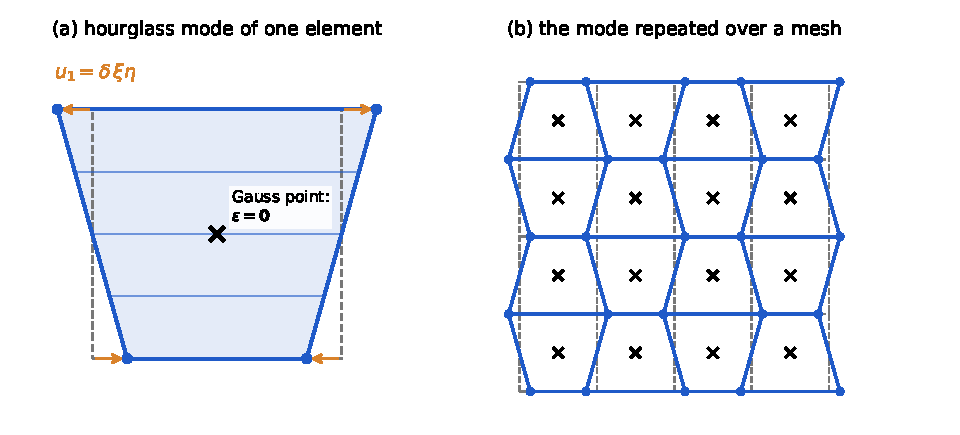
\includegraphics[width=0.85\textwidth]{figures/ch2/hourglass.pdf}
\caption{Hourglass mode of a bilinear square integrated with one Gauss point
(cross). (a) The nodal displacements $\pm\delta$ deform the element, but the
strain vanishes at the centre. (b) The same mode with alternating signs is a
zero-energy mode of the whole mesh.}
\label{fig:hourglass}
\end{figure}

\exercise{A bar in tension by the Ritz method}\label{exo:bar}
A bar of length $L$, section $A$ and modulus $E$ is clamped at $x=0$, loaded by
a uniform axial force $f$ per unit length and by a force $F$ at $x=L$. (a) Write
the potential energy and the exact solution. (b) Ritz with $w_1=x$. (c) Ritz
with $w_1=x$, $w_2=x^2$. Compare the end displacements and the energies.
\begin{solution}
(a) $\displaystyle \mathcal U_p(v)=\int_0^L\tfrac12EA(v')^2-\int_0^Lfv-Fv(L)$, $v(0)=0$;
Euler--Lagrange: $-EAu''=f$, $EAu'(L)=F$, so
$\displaystyle u=\frac{(F+fL)x-fx^2/2}{EA}$, $\displaystyle u(L)=\frac{FL+fL^2/2}{EA}$.
(b) $v=\alpha x$: $\mathcal U_p=\tfrac12EAL\alpha^2-\alpha(fL^2/2+FL)$, so
$\alpha=(F+fL/2)/EA$ and $v(L)=u(L)$ exactly, but the strain $\alpha$ is
constant: the stress is the average of the exact one. The energy is higher
than the exact one by $\displaystyle \frac{f^2L^3}{24EA}$.
(c) The exact solution belongs to the trial space, so the Ritz method
returns it: the Ritz solution is the best approximation in energy norm.
Figure~\ref{fig:bar-ritz} shows the three solutions for $F=0$: the
one-term displacement is exact only at the end, and its constant normal
force is the average of the exact one.
\end{solution}
\begin{figure}[h]
\centering
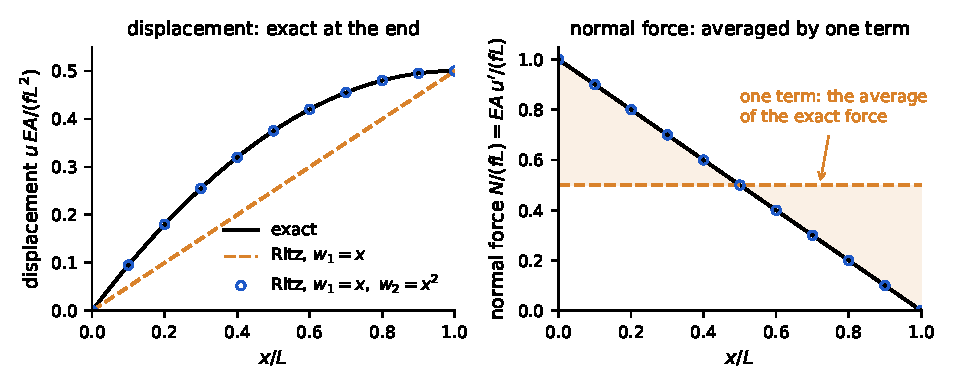
\includegraphics[width=0.9\textwidth]{figures/ch2/bar_ritz.pdf}
\caption{Ritz solutions of the bar of Exercise~\ref{exo:bar} under a uniform
load $f$, free end ($F=0$). Left: displacement. Right: normal force
$N=EA\,u'$. One term ($w_1=x$) gives a constant force, the average of the
exact one; two terms ($w_1=x$, $w_2=x^2$) give the exact solution.}
\label{fig:bar-ritz}
\end{figure}

\exercise{Why not polynomials?}\label{exo:conditioning}
For the bar of Exercise~\ref{exo:bar} with $EA=L=1$, use the monomials
$w_m=x^m$, $m=1,\dots,n$. Compute $\displaystyle K_{m\ell}=\int_0^1w_m'w_\ell'$ and its
condition number for $n=3,5,7,9$. Compare with $n$ hat functions.
\begin{solution}
$K_{m\ell}=m\ell/(m+\ell-1)$, a Hilbert-like matrix. Its condition numbers are
\begin{center}\renewcommand{\arraystretch}{1.1}
\begin{tabular}{lcccc}
\toprule
$n$ & 3 & 5 & 7 & 9\\
\midrule
monomials $x^m$ & $2.8\times10^2$ & $1.9\times10^5$ & $1.7\times10^8$ & $1.6\times10^{11}$\\
hat functions & $16.4$ & $45.5$ & $87.6$ & $142.7$\\
\bottomrule
\end{tabular}
\end{center}
\lstinputlisting[firstline=4]{python/examples/ch2/exo_conditioning.py}
The condition number of the monomial basis grows geometrically, by a factor
of about $30$ per function: from $n=12$ on it exceeds the inverse of the
machine precision, and the computed coefficients are meaningless
(Figure~\ref{fig:conditioning}). That of the finite element basis grows like
$1/h^2=n^2$.
\begin{figure}[h]
\centering
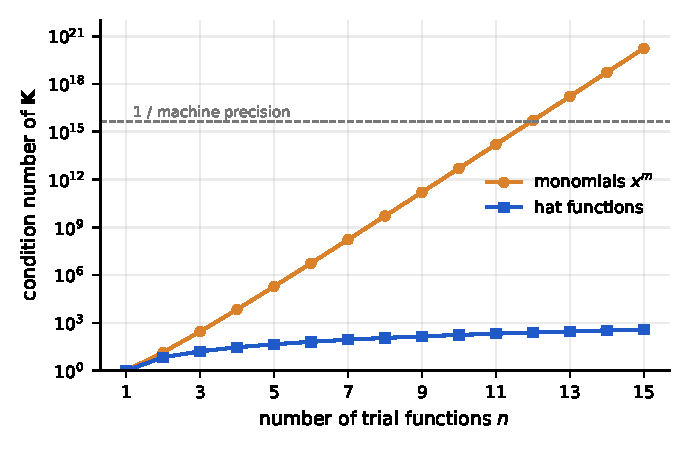
\includegraphics[width=0.6\textwidth]{figures/ch2/conditioning.pdf}
\caption{Condition number of the stiffness matrix of the bar against the
number of trial functions: monomials (geometric growth) and hat functions
(growth like $n^2$). Dashed: the inverse of the double-precision machine
epsilon.}
\label{fig:conditioning}
\end{figure}
\end{solution}

\exercise{A plate with a hole: Kirsch against finite elements}\label{exo:kirsch}
\index{Kirsch problem}\index{stress concentration}\index{finite element method!test against a closed-form solution}%
An infinite plate with a circular hole of radius $a$ carries a remote uniaxial
tension $\sigma$ along $\ve_1$ (plane stress or plane strain). In polar
coordinates $(r,\theta)$, with $\theta$ measured from $\ve_1$, the solution of
Kirsch~\cite{Kirsch1898} is
\begin{align*}
  \sigma_{rr}&=\frac\sigma2\Bigl(1-\frac{a^2}{r^2}\Bigr)
  +\frac\sigma2\Bigl(1-4\frac{a^2}{r^2}+3\frac{a^4}{r^4}\Bigr)\cos2\theta,\\
  \sigma_{\theta\theta}&=\frac\sigma2\Bigl(1+\frac{a^2}{r^2}\Bigr)
  -\frac\sigma2\Bigl(1+3\frac{a^4}{r^4}\Bigr)\cos2\theta,\qquad
  \sigma_{r\theta}=-\frac\sigma2\Bigl(1+2\frac{a^2}{r^2}-3\frac{a^4}{r^4}\Bigr)\sin2\theta .
\end{align*}
(a) Check the boundary conditions on the hole and at infinity. Give
$\sigma_{\theta\theta}$ on the hole and the stress concentration factor.
(b) Give $\sigma_{11}$ on the ligament $x_1=0$. At which distance from the hole
is it within $10\%$ of $\sigma$?
(c) Write a finite element program with linear triangles for a quarter of a
square plate of side $40a$: symmetry conditions $u_1=0$ on $x_1=0$ and $u_2=0$
on $x_2=0$, traction $\sigma\ve_1$ on the edge $x_1=20a$, a mesh graded
towards the hole. Compare with Kirsch on the hole and on the ligament, and
refine the mesh.
(d) Repeat the computation with a general finite element code, for instance
Cast3M or FEniCS, with linear and quadratic triangles, and compare the
meshes needed for a $1\%$ accuracy on the concentration factor.
\begin{solution}
(a) At $r=a$: $\sigma_{rr}=\tfrac\sigma2(1-4+3)\cos2\theta=0$ and
$\sigma_{r\theta}=-\tfrac\sigma2(1+2-3)\sin2\theta=0$: the hole is free. As
$r\to\infty$: $\sigma_{rr}\to\sigma\cos^2\theta$,
$\sigma_{\theta\theta}\to\sigma\sin^2\theta$,
$\sigma_{r\theta}\to-\sigma\sin\theta\cos\theta$, the polar components of
$\sigma\,\ve_1\otimes\ve_1$. On the hole
$\sigma_{\theta\theta}=\sigma(1-2\cos2\theta)$: $-\sigma$ at $\theta=0$ and
$3\sigma$ at $\theta=\pm\tfrac\pi2$. The concentration factor is $3$,
independent of the radius and of the elastic constants.
(b) On $x_1=0$, $\theta=\tfrac\pi2$ and $\sigma_{11}=\sigma_{\theta\theta}
=\sigma\bigl(1+\tfrac12a^2/x_2^2+\tfrac32a^4/x_2^4\bigr)$. With $t=a^2/x_2^2$,
$\tfrac12t+\tfrac32t^2=0.1$ gives $t=0.141$, $x_2=2.7a$: the perturbation
is local (Saint-Venant).
(c) The program below meshes the quarter plate with $n_\theta$ cells along
the hole and cells of nearly square shape growing geometrically away from it,
assembles the stiffness of linear triangles in plane stress, and averages the
element stresses at the nodes. It prints
\begin{center}\renewcommand{\arraystretch}{1.1}
\begin{tabular}{lcccc}
\toprule
$n_\theta$ & 12 & 24 & 48 & 96\\
\midrule
degrees of freedom & 624 & 2352 & 9120 & 35712\\
$\sigma_{11}(0,a)/\sigma$ (Kirsch: $3$) & 2.970 & 3.013 & 3.020 & 3.021\\
$\sigma_{22}(a,0)/\sigma$ (Kirsch: $-1$) & $-0.722$ & $-0.871$ & $-0.946$ & $-0.982$\\
\bottomrule
\end{tabular}
\end{center}
The concentration factor converges to $3.02$, not $3$: the plate is finite.
With a side of $160a$ the same mesh density gives $3.00$. The compressive
value at $\theta=0$ converges more slowly: there the hoop stress drops from
$-\sigma$ to $-0.6\sigma$ within $0.1a$, and the nodal average of constant
element stresses smooths this gradient. Figure~\ref{fig:kirsch} compares the
fields for $n_\theta=48$.
\lstinputlisting[firstline=4]{python/examples/ch2/kirsch_fem.py}
(d) Both codes follow the same steps: mesh, symmetry conditions, traction on
the edge, solution, nodal stresses on the hole. Quadratic triangles represent
the linear variation of the stress inside each element, and reach the same
accuracy with far fewer degrees of freedom.
\end{solution}
\begin{figure}[h]
\centering
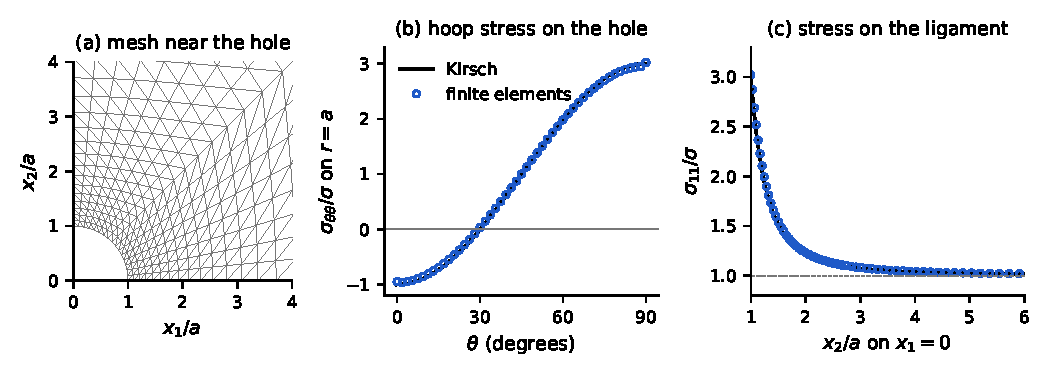
\includegraphics[width=\textwidth]{figures/ch2/kirsch.pdf}
\caption{Plate with a hole under remote tension $\sigma$ (Exercise~\ref{exo:kirsch}),
linear triangles, $48$ cells along the quarter hole. (a) The mesh near the
hole (shown coarser). (b) Hoop stress on the hole: from $-\sigma$ to the
concentration $3\sigma$. (c) $\sigma_{11}$ on the ligament $x_1=0$: the
perturbation decays within a few radii.}
\label{fig:kirsch}
\end{figure}

%======================================================================
\begin{chapterbib}{99}
\bibitem{BonnetFrangi2007} M.~Bonnet, A.~Frangi, \emph{Analyse des solides d\'eformables par la m\'ethode des \'el\'ements finis}, \'Editions de l'\'Ecole Polytechnique, 2007.
\bibitem{Chadwick2001} P.~Chadwick, M.~Vianello, S.~C.~Cowin, A new proof that the number of linear elastic symmetries is eight, \emph{J. Mech. Phys. Solids} 49 (2001) 2471--2492.
\bibitem{Coirier1997} J.~Coirier, \emph{M\'ecanique des milieux continus}, Dunod, 1997.
\bibitem{Crank1975} J.~Crank, \emph{The Mathematics of Diffusion}, 2nd ed., Oxford University Press, 1975.
\bibitem{ConstantinescuKorsunsky2007} A.~Constantinescu, A.~Korsunsky, \emph{Elasticity with Mathematica}, Cambridge University Press, 2007.
\bibitem{CottrellHughesBazilevs2009} J.~A.~Cottrell, T.~J.~R.~Hughes, Y.~Bazilevs, \emph{Isogeometric Analysis: Toward Integration of CAD and FEA}, Wiley, 2009.
\bibitem{FreezeCherry} R.~A.~Freeze, J.~A.~Cherry, \emph{Groundwater}, Prentice-Hall, 1979.
\bibitem{Germain1983} P.~Germain, \emph{M\'ecanique des milieux continus}, Masson, 1983.
\bibitem{HughesCottrellBazilevs2005} T.~J.~R.~Hughes, J.~A.~Cottrell, Y.~Bazilevs, Isogeometric analysis: CAD, finite elements, NURBS, exact geometry and mesh refinement, \emph{Comput. Methods Appl. Mech. Engrg.} 194 (2005) 4135--4195.
\bibitem{Hughes1987} T.~J.~R.~Hughes, \emph{The Finite Element Method}, Prentice Hall, 1987.
\bibitem{IncroperaDeWitt} F.~P.~Incropera, D.~P.~DeWitt, T.~L.~Bergman, A.~S.~Lavine, \emph{Fundamentals of Heat and Mass Transfer}, 6th ed., Wiley, 2007.
\bibitem{Kirsch1898} E.~G.~Kirsch, Die Theorie der Elastizit\"at und die Bed\"urfnisse der Festigkeitslehre, \emph{Zeitschrift des Vereines deutscher Ingenieure} 42 (1898) 797--807.
\bibitem{Nye1985} J.~F.~Nye, \emph{Physical Properties of Crystals: Their Representation by Tensors and Matrices}, Oxford University Press, 1957; revised edition 1985.
\bibitem{Salencon2001} J.~Salen\c{c}on, \emph{Handbook of Continuum Mechanics: General Concepts, Thermoelasticity}, Springer, 2001.
\bibitem{SoutasLittle1973} R.~W.~Soutas-Little, \emph{Elasticity}, Dover, 1973.
\bibitem{StrangAM} G.~Strang, \emph{Introduction to Applied Mathematics}, Wellesley-Cambridge Press, 1986.
\end{chapterbib}
